%==============================================================================
% tento soubor pouzijte jako zaklad
% this file should be used as a base for the thesis
% Autoři / Authors: 2008 Michal Bidlo, 2016 Jaroslav Dytrych
% Kontakt pro dotazy a připomínky: dytrych@fit.vutbr.cz
% Contact for questions and comments: dytrych@fit.vutbr.cz
%==============================================================================
% kodovani: UTF-8 (zmena prikazem iconv, recode nebo cstocs)
% encoding: UTF-8 (you can change it by command iconv, recode or cstocs)
%------------------------------------------------------------------------------
% zpracování / processing: make, make pdf, make clean
%==============================================================================
% Soubory, které je nutné upravit: / Files which have to be edited:
%   projekt-20-literatura-bibliography.bib - literatura / bibliography
%   projekt-01-kapitoly-chapters.tex - obsah práce / the thesis content
%   projekt-30-prilohy-appendices.tex - přílohy / appendices
%==============================================================================
%\documentclass[]{fitthesis} % bez zadání - pro začátek práce, aby nebyl problém s překladem
%\documentclass[english]{fitthesis} % without assignment - for the work start to avoid compilation problem
%\documentclass[zadani]{fitthesis} % odevzdani do wisu - odkazy jsou barevné
%\documentclass[english,zadani]{fitthesis} % for submission to the IS FIT - links are color
\documentclass[zadani,print]{fitthesis} % pro tisk - odkazy jsou černé
%\documentclass[zadani,cprint]{fitthesis} % pro barevný tisk - odkazy jsou černé, znak VUT barevný
%\documentclass[english,zadani,print]{fitthesis} % for the color print - links are black
%\documentclass[english,zadani,cprint]{fitthesis} % for the print - links are black, logo is color
% * Je-li práce psaná v anglickém jazyce, je zapotřebí u třídy použít
%   parametr english následovně:
%   If thesis is written in english, it is necessary to use
%   parameter english as follows:
%      \documentclass[english]{fitthesis}
% * Je-li práce psaná ve slovenském jazyce, je zapotřebí u třídy použít
%   parametr slovak následovně:
%   If the work is written in the Slovak language, it is necessary
%   to use parameter slovak as follows:
%      \documentclass[slovak]{fitthesis}
% * Je-li práce psaná v anglickém jazyce se slovenským abstraktem apod.,
%   je zapotřebí u třídy použít parametry english a enslovak následovně:
%   If the work is written in English with the Slovak abstract, etc.,
%   it is necessary to use parameters english and enslovak as follows:
%      \documentclass[english,enslovak]{fitthesis}

% Základní balíčky jsou dole v souboru šablony fitthesis.cls
% Basic packages are at the bottom of template file fitthesis.cls
% zde můžeme vložit vlastní balíčky / you can place own packages here

% Kompilace po částech (rychlejší, ale v náhledu nemusí být vše aktuální)
% Compilation piecewise (faster, but not all parts in preview will be up-to-date)
% \usepackage{subfiles}

% Nastavení cesty k obrázkům
% Setting of a path to the pictures
%\graphicspath{{obrazky-figures/}{./obrazky-figures/}}
%\graphicspath{{obrazky-figures/}{../obrazky-figures/}}

%---rm---------------
\renewcommand{\rmdefault}{lmr}%zavede Latin Modern Roman jako rm / set Latin Modern Roman as rm
%---sf---------------
\renewcommand{\sfdefault}{qhv}%zavede TeX Gyre Heros jako sf
%---tt------------
\renewcommand{\ttdefault}{lmtt}% zavede Latin Modern tt jako tt

% vypne funkci šablony, která automaticky nahrazuje uvozovky,
% aby nebyly prováděny nevhodné náhrady v popisech API apod.
% disables function of the template which replaces quotation marks
% to avoid unnecessary replacements in the API descriptions etc.
\csdoublequotesoff

% =======================================================================
% balíček "hyperref" vytváří klikací odkazy v pdf, pokud tedy použijeme pdflatex
% problém je, že balíček hyperref musí být uveden jako poslední, takže nemůže
% být v šabloně
% "hyperref" package create clickable links in pdf if you are using pdflatex.
% Problem is that this package have to be introduced as the last one so it
% can not be placed in the template file.
\ifWis
\ifx\pdfoutput\undefined % nejedeme pod pdflatexem / we are not using pdflatex
\else
  \usepackage{color}
  \usepackage[unicode,colorlinks,hyperindex,plainpages=false,pdftex]{hyperref}
  \definecolor{links}{rgb}{0.4,0.5,0}
  \definecolor{anchors}{rgb}{1,0,0}
  \def\AnchorColor{anchors}
  \def\LinkColor{links}
  \def\pdfBorderAttrs{/Border [0 0 0] }  % bez okrajů kolem odkazů / without margins around links
  \pdfcompresslevel=9
\fi
\else % pro tisk budou odkazy, na které se dá klikat, černé / for the print clickable links will be black
\ifx\pdfoutput\undefined % nejedeme pod pdflatexem / we are not using pdflatex
\else
  \usepackage{color}
  \usepackage[unicode,colorlinks,hyperindex,plainpages=false,pdftex,urlcolor=black,linkcolor=black,citecolor=black]{hyperref}
  \definecolor{links}{rgb}{0,0,0}
  \definecolor{anchors}{rgb}{0,0,0}
  \def\AnchorColor{anchors}
  \def\LinkColor{links}
  \def\pdfBorderAttrs{/Border [0 0 0] } % bez okrajů kolem odkazů / without margins around links
  \pdfcompresslevel=9
\fi
\fi
% Řešení problému, kdy klikací odkazy na obrázky vedou za obrázek
% This solves the problems with links which leads after the picture
\usepackage[all]{hypcap}

% Informace o práci/projektu / Information about the thesis
%---------------------------------------------------------------------------
\projectinfo{
  %Prace / Thesis
  project={BP},            %typ práce BP/SP/DP/DR  / thesis type (SP = term project)
  year={2018},             % rok odevzdání / year of submission
  date=\today,             % datum odevzdání / submission date
  %Nazev prace / thesis title
  title.cs={Rozšíření systému pro získávání, zpracování a analýzu rozsáhlých kolekcí textů z webu},  % název práce v češtině či slovenštině (dle zadání) / thesis title in czech language (according to assignment)
  title.en={Extending System for Acquiring, Processing, and Analysing Large Web Text Collections}, % název práce v angličtině / thesis title in english
  %title.length={14.5cm}, % nastavení délky bloku s titulkem pro úpravu zalomení řádku (lze definovat zde nebo níže) / setting the length of a block with a thesis title for adjusting a line break (can be defined here or below)
  %Autor / Author
  author.name={Jiří},   % jméno autora / author name
  author.surname={Matějka},   % příjmení autora / author surname
  %author.title.p={Bc.}, % titul před jménem (nepovinné) / title before the name (optional)
  %author.title.a={Ph.D.}, % titul za jménem (nepovinné) / title after the name (optional)
  %Ustav / Department
  department={UPGM}, % doplňte příslušnou zkratku dle ústavu na zadání: UPSY/UIFS/UITS/UPGM / fill in appropriate abbreviation of the department according to assignment: UPSY/UIFS/UITS/UPGM
  % Školitel / supervisor
  supervisor.name={Pavel},   % jméno školitele / supervisor name
  supervisor.surname={Smrž},   % příjmení školitele / supervisor surname
  supervisor.title.p={Doc. RNDr.},   %titul před jménem (nepovinné) / title before the name (optional)
  supervisor.title.a={Ph.D.},    %titul za jménem (nepovinné) / title after the name (optional)
  % Klíčová slova / keywords
  keywords.cs={web, stahování webových stránek, korpus, vertikální text, extrakce textu z HTML kódu, analýza textu}, % klíčová slova v českém či slovenském jazyce / keywords in czech or slovak language
  keywords.en={web, web pages downloading, corpus, text in vertical format, text extraction from HTML code, text analysis}, % klíčová slova v anglickém jazyce / keywords in english
  % Abstrakt / Abstract
  abstract.cs={Cílem práce je rozšířit stávající systém pro kolekci, stahování, zpracování a analýzu webových stránek. Práce se zabývá automatizací veškeré prováděné činosti, přináší nové nástroje do stávajícího systému a nabízí nejen nové verze některých nástrojů zapojených do systému zpracování, ale nabízí i nové postupy a myšlenky.}, % abstrakt v českém či slovenském jazyce / abstract in czech or slovak language
  abstract.en={The aim of the thesis is to extend the existing system for collecting, downloading, processing and analyzing web pages. This work deals with the automation of all processes, brings new tools into the existing system and offers new versions of some tools involved in the processing system and also offers new procedures and ideas.}, % abstrakt v anglickém jazyce / abstract in english
  % Prohlášení (u anglicky psané práce anglicky, u slovensky psané práce slovensky) / Declaration (for thesis in english should be in english)
  declaration={Prohlašuji, že jsem tuto bakalářskou práci vypracoval samostatně pod vedením pana Pavla Smrže, doc. RNDr., Ph.D. Uvedl jsem všechny literární prameny a publikace, ze kterých jsem čerpal.},
  %declaration={Hereby I declare that this bachelor's thesis was prepared as an original author’s work under the supervision of Mr. X
% The supplementary information was provided by Mr. Y
% All the relevant information sources, which were used during preparation of this thesis, are properly cited and included in the list of references.},
  % Poděkování (nepovinné, nejlépe v jazyce práce) / Acknowledgement (optional, ideally in the language of the thesis)
  acknowledgment={Tímto bych chtěl poděkovat všem, kteří se na mé práci podíleli nebo mi byly oporou, především panu docentu Pavlu Smržovi a panu doktoru Jaroslavu Dytrychovi nejen za cennou pomoc, ale i za možnost zapojit se do tohoto projektu.},
  %acknowledgment={Here it is possible to express thanks to the supervisor and to the people which provided professional help
%(external submitter, consultant, etc.).},
  % Rozšířený abstrakt (cca 3 normostrany) - lze definovat zde nebo níže / Extended abstract (approximately 3 standard pages) - can be defined here or below
  %extendedabstract={Do tohoto odstavce bude zapsán rozšířený výtah (abstrakt) práce v českém (slovenském) jazyce.},
  %faculty={FIT}, % FIT/FEKT/FSI/FA/FCH/FP/FAST/FAVU/USI/DEF
  faculty.cs={Fakulta informačních technologií}, % Fakulta v češtině - pro využití této položky výše zvolte fakultu DEF / Faculty in Czech - for use of this entry select DEF above
  faculty.en={Faculty of Information Technology}, % Fakulta v angličtině - pro využití této položky výše zvolte fakultu DEF / Faculty in English - for use of this entry select DEF above
  department.cs={Ústav počítačové grafiky a multimédií}, % Ústav v češtině - pro využití této položky výše zvolte ústav DEF nebo jej zakomentujte / Department in Czech - for use of this entry select DEF above or comment it out
  department.en={Department of Computer Graphics and Multimedia} % Ústav v angličtině - pro využití této položky výše zvolte ústav DEF nebo jej zakomentujte / Department in English - for use of this entry select DEF above or comment it out
}

% Rozšířený abstrakt (cca 3 normostrany) - lze definovat zde nebo výše / Extended abstract (approximately 3 standard pages) - can be defined here or above
%\extendedabstract{Do tohoto odstavce bude zapsán výtah (abstrakt) práce v českém (slovenském) jazyce.}

% nastavení délky bloku s titulkem pro úpravu zalomení řádku - lze definovat zde nebo výše / setting the length of a block with a thesis title for adjusting a line break - can be defined here or above
%\titlelength{14.5cm}


% řeší první/poslední řádek odstavce na předchozí/následující stránce
% solves first/last row of the paragraph on the previous/next page
\clubpenalty=10000
\widowpenalty=10000

\begin{document}
  % Vysazeni titulnich stran / Typesetting of the title pages
  % ----------------------------------------------
  \maketitle
  % Obsah
  % ----------------------------------------------
  \setlength{\parskip}{0pt}

  {\hypersetup{hidelinks}\tableofcontents}

  % Seznam obrazku a tabulek (pokud prace obsahuje velke mnozstvi obrazku, tak se to hodi)
  % List of figures and list of tables (if the thesis contains a lot of pictures, it is good)
  \ifczech
    \renewcommand\listfigurename{Seznam obrázků}
  \fi
  \ifslovak
    \renewcommand\listfigurename{Zoznam obrázkov}
  \fi
  % \listoffigures

  \ifczech
    \renewcommand\listtablename{Seznam tabulek}
  \fi
  \ifslovak
    \renewcommand\listtablename{Zoznam tabuliek}
  \fi
  % \listoftables

  \ifODSAZ
    \setlength{\parskip}{0.5\bigskipamount}
  \else
    \setlength{\parskip}{0pt}
  \fi

  % vynechani stranky v oboustrannem rezimu
  % Skip the page in the two-sided mode
  \iftwoside
    \cleardoublepage
  \fi

  % Text prace / Thesis text
  % ----------------------------------------------
  %=========================================================================
% (c) Michal Bidlo, Bohuslav Křena, 2008

\chapter{Úvod}
Na úvod mé práce uvedu několik důvodů, proč se zajímám o~problematiku zpracování
rozsáhlých kolekcí textů z~webu a~také uvedu čtenáře do problematiky.

V~následující kapitole bude uvedeno několik zajímavých příkladů použití korpusů ve světě.
Protože korpusů existuje obrovské množství, byly vybrány ty provedení, která mi přišla
nejzajímavější.

Další kapitoly jsou věnovány mé práci. Kapitoly jsou rozděleny podle jednotlivých částí celkového
systému zpracování. V~každé z~těchto kapitol se nachází podrobnější popis
problematiky a~jejího řešení, použité nástroje a~na závěr je porovnání
s~původním systémem.

V~přílohách je poté možné vyčíst různé údaje o~výkonostní náročnosti projektu a~srovnání s~původním systémem,
stručný postup jak tvořit obslužné skripty k~vytvořeným knihovnám a~samotné úkázky jednotlivých kroků zpracování.

\section{Volba tématu}
Téma Rozšíření systému pro získávání, zpracování a~analýzu rozsáhlých kolekcí textů z~webu
jsem si zvolil hlavně z~důvodu své dvouleté spolupráci s~výzkumnou skupinou KNOT~\cite{KNOT}, svému zájmu a~svým zkušenostem v~této problematice.

\section{Úvod do problematiky}
Cílem tohoto projektu není vytvořit nový proces zpracování webových korpusů, ale rozšířit stávající
systém. Aktuálně dokážeme jednorázově vytvořit korpus a~sémanticky ho označit. Problém tedy není v~tom,
že korpus nelze vytvořit, ale že to nelze provádět automaticky. To znamená, že do procesu musí vstoupit
člověk, který je obeznámen s~nástroji i problematikou, spustit mnoho nástrojů ve správném pořadí a~sledovat, zda při zpracování nenastane chyba.

Dalšími problémemy jsou rozmanitost webových stránek, jak z~hlediska vzhledu, jejich účelu, tak i
způsobu, jak je zdrojový kód stránky napsán. Dalším faktorem ovlivňující obtížnost je tolerance jazyka HTML k~chýbám
Vícejazyčnost stránek nutí použití dalších nástrojů pro detekci jazyka, které zpomalují celkové zpracování
a~tyto nástroje jsou často mateny ne tolik gramatickými chybami, jako spíše příliš krátkými textovými úseky,
jakým může být například komentář uživatele k~jednomu ze článků na webové stránce.

Webových zdrojů je obrovské množství a~je nemožné, nebo přinejmenším velice obtížné, napsat optimální program
pro všechny webové stránky. Má práce se zaměřuje zejména na zpracování článků v~českých mediích. Velké množství těchto zdrojů
je logicky členěno do bloků, ale je zde i mnoho reklam. HTML kód je často bez chyb a~lze ho poměrně jednoduše
zpracovat, ale jsou zde i skutečnosti, na které je potřeba si dát pozor.

\section{Definice základních pojmů}
Pro úplné porozumnění textu je potřeba znát mnoho odborných termínů. Většina termínů je vysvětlena
v~jednotlivých kapitolách, ale nachází se zde několik termínů, které je třeba vysvětlit předem.

\subsection{Tokenizace}
\label{Tokenizace}
Tokenizace je proces, kde je sekvence znaků rozdělena na tzv. \textit{tokeny} (žetony). Tyto \textit{tokeny} jsou
často označovány jako slova nebo výrazy. Jinýmy slovy, jedná se o~proces, kde se užitečný text rozdělý na slova~\cite{TOKENIZACE}.

\subsection{Tagging}
\label{Tagging}
Tagging je proces, ve kterém se pracuje s~jednotlivými slovy. V~tomto procesu se provádí morfologický rozbor daného slova,
zařazuje se do gramatické kategorie a~určuje se jeho základní tvar~\cite{TAGGING}.

\subsection{Parsing}
\label{Parsing}
Parsing je proces zpracování věty. Je to proces podobný větnému rozboru, kde se hledají vztahy mezi jednotlivými slovy
ve větě.

\chapter{Zpracování webových korpusů ve světě}
Korpusy obsahují obrovské množství dat a~jsou cennými informačními zdroji. Se samotnými korpusy
lze provádět spoustu činností. S~dostatečně velkou databází lze lépe porozumět jazyku
(zjistit, jak se jazyk v~průběhu let mění, jaká slova jsou nejčastěji používaná, atd.),
provádět výzkumy (jaké jsou trendy ve společnosti, jak dokáže určitá událost ovlivnit svět okolo sebe apod.),
tvořit vyhledávače a~spoustu dalších věcí. Z~toho plyne, že se tvoří spousta korpusů.

Častým zdrojem dat pro tvorbu korpusů jsou webové stránky. Podle statistik se
každý týden se zaregistruje přibližně 800 000 -- 1 100 000 nových domén~\cite{NEWPAGES},
což je obrovské množství dat, která jsou potenciálně vhodná pro tvorbu webového korpusu.

V~této kapitole bude pojednáno o~některých zajímavých postupech tvorby korpusových dat
a~práce s~nimi.

\section{ClueWeb09 corpus}
\label{ClueWeb09}
Jedná se o~poměrně rozsáhlý webový korpus určený pro podporu výzkumu vyhledávácích informací
a~vývoj technologií zabývající se zpracováním lidských jazyků. Tento korpus obsahuje zhruba
jednu miliardu webových stránek, jeho komprimovaná velikost je 5 TB (po dekompresi velikost
dosahuje až 25 TB). V~korpusu je obsažen text v~deseti různých jazycích.

Jednotlivé webové stránky jsou ukládány v~souborech ve fromátu WARC~(\ref{warc_format}).
Každá z~těchto kolekcí stránek obsahuje několik desítek tisíc stránek (většinou okolo 40 000 stránek) a~komprimovaná
nástrojem gzip.

Informace obsažené v~této kapitole byly získány z~webových stránek projektu~\cite{CLUEWEB}.

\section{Common Crawl corpus}
\label{commoncrawl}
\textit{Common Crawl corpus} je volně dostupným webovým korpusem spravovaný neziskovou organizací
\textit{The Common Crawl Foundation}. Aktuální velikost korpusu se pohybuje v~řádech petabajtů a~jsou zde obsaženy webové stránky stažené za posledních 7 let. Tebto korpus obsahuje miliardy
webových stránek ve více než 40 jazycích.

Informace obsažené v~této kapitole byly získány z~webových stránek projektu~\cite{COMMONCRAWL}.

\section{ChatNoir}
\textit{ChatNoir}, francouzky černá kočka, je vyhledávačem, který pracuje nad korpusovými daty. Korpus,
který byl k~tvorbě tohoto vyhledávače použit, je anglickou podmnožinou dat korpusu \textit{ClueWeb09 corpus}~(\ref{ClueWeb09}) (anglická podmnožina obsahuje 500 milionů stránek s~celkovou veliksotí 12 TB )~\cite{CHATNOIR}.
Dalším z~použitých zdrojů dat je rozsáhlý webový korpus \textit{Common Crawl corpus}~(\ref{commoncrawl})~\cite{COMMONCRAWL_EXAMPLES}.

Projekt \textit{ChatNoir} je psán převážně v~jazyku Java a~v~procesu je, kromě jiného, zapojeno získání textu
z~HTML stránek, detekcí jazyka a~tvorba indexů pro vyhledávač~\cite{CHATNOIR_GIT}.

\section{Google Ngram corpus}
Tento korpus obsahuje 500 miliard slov z~5,2 miliónu knih, které vyšly za posledních 500 let.
Data byla získána z~knih psaných v~angličtině, francouštině, čínštině, ruštině,
španělštině a~němčině. Nad tímto korpusem byl posléze postaven nástroj, který
je schopen měřit frekvenci používání různých slov v~průběhu let~\cite{NGRAM}.

\chapter{Kolekce odkazů a~stahování webových stránek} % idealne 5 stran
Aby bylo možné zpracovat webové články, je nutné mít k~dispozici alespoň minimum dat. Způsobů, pomocí kterých lze získávat pravidelně nové webové
články, je více. Oblíbeným je například klasický webcrawling, kde se ze stažené stránky extrahují odkazy a~získané adresy se použijí k~dalšímu sběru dat. Má práce se zaměřuje hlavně na využití technologií RSS a~ATOM.

RSS \textit{Rich Site Summary} je technologie sloužící k~syndikaci obsahu. Využívá XML formátu a~uživatelé
webových stránek si mohou díky této technologii nastavit odběr novinek z~webu~\cite{RSS}. Zejména díky tomu, že technologie RSS neměla ve
své době téměř žádnou konkurenci, rychle se rozšířila a~ještě dnes je nejpoužívanějším nástrojem, přestože je vývoj od roku 2003
zastaven~\cite{ATOM_VS_RSS}.

ATOM \textit{Atom Syndication Format} je jedním z~webových standardů. Podobně, jako RSS, se využívá XML formátu a~slouží
k~informování uživatelů stránek o~nových článcích~\cite{ATOM}. Na rozdíl od RSS se jedná o~mladší formát a~už od začátku se dbalo na
modularitu, znovupoužitelnost a~přehlednost kódu. Zatímco RSS není IETF standardem, ATOM sem byl zařazen v~prosinci roku 2005~\cite{ATOM_VS_RSS}.

\section{Zpracování RSS a~ATOM souborů}
Jak RSS, tak i ATOM jsou psané pomocí jazyka XML. Proto byl použit modul \linebreak\textit{xml.etree.ElementTree} určený k~práci nad jednotlivými
elementy. Ovšem ne všechny zpracovávané dokumenty jsou bez chyb a~právě na tyto dokumenty je výše zmíněný modul krátký. U~poškozených
dokumentů zpracování probíhá pomocí regulárních výrazů a~díky tomu lze získat alespoň pár odkazů na nové články.

\section{Použité nástroje}
Kolekce odkazů a~stahování stránek je implementována v~jazyce Python. Konkrétní verze jazyka je Python3.5, která je nainstalovaná na serverech,
na nichž budou nástroje spuštěny. Jazyk Python byl zvolen nejen kvůli popularitě a~velkému množství knihoven, ale i kvůli nenáročnosti
procesu kolekce a~stahování stránek na procesor.

\subsection{Urllib}
\label{urllib}
Urllib je balíček několika modulů určených pro práci s~url. V~této práci bylo využito pouze modulu \textit{urllib.request},
který je určený ke stahování webových zdrojů pomocí url odkazu~\cite{URLLIB}. Pomocí tohoto modulu se podařilo stáhnout většinu
odkazů, ale stále zde bylo několik stránek, které se podařilo stáhnout až na pozdější pokus a~také zde byly stránky, které
se stáhnout nepodařilo, přestože přes prohlížeč na ně přistoupit bylo možné. Tento problém vyřešil nástroj \textit{GNU Wget}.

\subsection{GNU Wget}
\label{wget}
\textit{GNU Wget} je aplikace pro stahování souborů pomocí protokolů HTTP, HTTPS, FTP a~FTPS. Je to neinteraktivní nástroj spouštěný uvnitř
příkazové řádky a~je vhodný pro použití v~automatických skriptech~\cite{WGET}. Pro spuštění této aplikace uvnitř skriptu využito knihovny \textit{subprocess}~(\ref{subprocess}).
Bohužel úplné nahrazení \textit{urrlib} aplikací \textit{GNU Wget} poměrně výrazně zpomalilo proces kolekce odkazů. Bylo nutné každé stránce dát určitý časový limit
na stažení. Většina stránek je stažena do 1 sekundy, ale pokud je zapotřebí stáhnout i zbylé stránky, které jsou umístěny na pomalejších, méně dostupných
nebo vzdálených serverech, je nezbytné časový limit zvýšit alespoň na 3 sekundy.

\subsection{Warc}
\label{warc}
\textit{Warc}, je knihovna pro jazyk Python umožňující práci se souborem uloženým ve formátu WARC~(\ref{warc_format}). Tato
značně zjednodušuje získání jednotlivých záznamů (v~tomto případě webových stránek) nebo tvorbu samotných souborů
formátu WARC~\cite{WARC}.

Pro účel stahování stránek zde byla tato knihovna použita právě za účelem tvorby souborů
typu warc.

\subsection{Lzma}
\label{lzma}
Modul \textit{lzma} nabízí třídy a~funkce určené pro kompresi a~dekompresi dat s~použitím algoritmu LZMA.
Součástí je také souborové rozhraní podporující souborové formáty \textit{.xz} a~\textit{.lzma}, které
používá aplikace xz~\cite{LZMA}.

Pro účely kolekce a~stahování dat je tento modul použit ke kompresi souborů.

\section{Paralelní přístup}
Jak bylo zmíněno výše, aplikace \textit{GNU Wget} nemohla úplně nahradit \textit{urllib} z~důvodu časové náročnosti. Proto byla zvolena zlatá střední cesta a~v~případě,
že \textit{urllib} selže, stránku se pokusila stáhnout aplikace \textit{GNU Wget}. Sice bylo dosaženo rychlejšího stahování, ale stále to nestačilo. Protože se ale většinu
času čeká na odpověď serveru a~proces je uspaný, byl zvolen paralelní přístup. Místo toho, aby na odpověď čekal jeden proces, čekalo na ni
hned několik procesů. K~paralelizaci bylo využito modulu \textit{concurrent.futures} a~celý proces kolekce a~stahování proces byl několikanásobně zrychlen. Veškerá rizika,
která s~sebou přináší paralelní zpracování, byla vyřešena přidělením maximální doby pro zpracování jednoho odkazu. Pokud rodič čekal příliš
dlouho na potomka, potomek byl zabit a~rodič pokračoval v~práci.


\section{Deduplikace}
Při zpracování rozsáhlých webových kolekcích je potřeba provádět deduplikaci dat. Každou staženou webovou stránku je potřeba zpracovat
dalšími nástroji a~to znamená, že jim musíme věnovat určitý procesorový čas. Navíc je zbytečné archivovat jednu a~tu samou stránku
vícekrát, proto je potřeba už při stahování článku dát důraz na to, abychom opakovaně nestáhli tutéž stránku znovu.
Je třeba si uvědomit, že v~této fázi celého procesu zpracování máme pouze odkazy a~jediný možný způsob deduplikace dat je zpracovat každý
odkaz právě jednou. V~novém systému se deduplikace řeší na úrovni kolekce odkazů. Kolektor odkazů si vede soubory, ve kterých jsou seznamy již
zpracovaných odkazů. Klade se přitom důraz na to, aby s~tímto souborem manipuloval vždy právě jeden kolektor a~sám kolektor si tyto soubory
u~sebe držel minimální dobu a~nedocházelo tak ke zbytečné ztrátě deduplikačních dat a~poté i tvorbě následných duplicit.

\section{Ukládání stažených dat}
Stažené stránky se dlouhodobě ukládají, a~proto je potřeba zvolit vhodnou formu komprese dat a~formát uložení jednotlivých záznamů.

\subsection{Komprese dat}
Dnes existuje spousta nástrojů umožňující
kompresi dat, k~obecně nejznámějším patří asi WinRAR, 7-zip nebo gzip. Použití WinRAR a~7-zip je přinejmenším nevhodné v~tomto projektu,
proto jsem se rozhodoval mezi výše zmíněným nástrojem gzip a~ne tolik známým xz. Oba nástroje mají své výhody.
Mezi výhody formátu xz patří menší výsledná velikost souborů, ovšem za cenu rychlosti. Formát gzip má na druhou stanu
relativně rychlou kompresi a~dekompresi dat~\cite{GZIP_VS_XZ}. Protože, jak již bylo zmíněno,
se stránky budou ukládat dlouhodobě, byl zvolen formát xz.

\subsection{WARC}
\label{warc_format}
Pro ukládání webových kolekcí je použit formát WARC (Web ARChive). Tento formát specifikuje metodu pro kombinaci
několika digitálních zdrojů do jednoho archivu spolu se souvisejícími informacemi~\cite{WARC_FROMAT}. Tento formát se často používá
pro webový crawling, a~proto byl i zvolen v~mé práci.

\section{Srovnání s~původním systémem}
V~této kapitole budete obeznámeni se základnímy prvky původního a~nového systému. Dále budete
obeznámeni s~jejich zásadními rozdíly.

\subsection{Původní systém}
Původní systém využíval stahování stránek pouze pomocí \textit{urllib}. Kolekci odkazů z~RSS a~Atom zdrojů zastávaly 2
skripty -- \textit{collect.py} a~\textit{download.py}. Skripty byly napsány v~jazyce Python verze Python2.7 pro projekt
Newsbrief eu~\cite{NEWSBRIEF}.

Kolekce odkazů byla implementována skriptem \textit{collect.py}. Samotná kolekce se spouštěla pomocí nástroje \textit{cron} každé
2 hodiny. Později byl skript přepsán do jazyka Python verze Python3.5 a~optimalizován. To vystačilo až do doby, než se začaly hromadit
RSS zdroje a~skript přestával stíhat sbírat odkazy z~RSS a~ATOM zdrojů. Stávalo se běžně, že v~jednu chvíli běželo najednou několik kolekcí odkazů
a~navzájem si přepisovaly deduplikační soubory a~tak se jedna stránka mohla stáhnout vícekrát. Tehdy přestal být tento nástroj vhodný
pro svůj účel.

O~stahování stránek se staral skript \textit{download.py}. Stejně jako \textit{collect.py}, i tento nástroj se spouštěl pravidelně
pomocí \textit{cronu}, pouze se namísto každých dvou hodin spouštěl jednou za 24 hodin. Skript byl následně přepsán do jazyka Python3.6,
z~důvodu chyby ve vertikalizátoru~(\ref{vertikalizator}).

\subsection{Nový systém}
Momentálně se, na rozdíl od předchozích nástrojů, stahují stránky paralelně. O~spouštění kolekce, stahování stránek, deduplikaci odkazů a~vedení statistik se
stará skript \textit{big\_brother.py}, který pravidelně spouští 2 skripty. Prvním z~nich je skript \textit{link\_collector.py}, využívající třídy \textit{Link\_collector}.
Tato třída je schopna vyhledat RSS a~ATOM zdroje na stažených stránkách a~extrahovat z~RSS a~ATOM souborů odkazy na nové články.
Navíc je tato třída přímým potomkem třídy \textit{Page\_downloader}, a~díky dědičnosti je schopna stahovat stránky jak sekvenčně, tak paralelně.

Stahování je řešeno skriptem \textit{page\_downloader.py}, který využívá třídy \textit{Page\_generator}. Tato třída je schopna se dotazovat jednotlivých serverů
s~časovým odstupem mezi dvěma dotazy na tentýž server a~stahovat z~nich stránky. Navíc je, stejně jako \textit{Link\_collector.py}, přímým potomkem
třídy \textit{Page\_downloader} a~získává tak možnost paralelního i sekvenčního stahování souborů ze serverů.

\chapter{Získání čistého textu ze stažených stránek}
\label{cisty_text}
Ve chvíli, kdy jsou k~dispozici data, lze započít další zpracování. Pro práci s~html souborem existuje celá řada nástrojů
programovaných v~mnoha jazycích, přesto ale je zde velké množství překážek.

\section{Problémy při zpracování webových stránek}
Jak již bylo dříve zmíněno, internet je velice rozmanitý a~existuje nespočet způsobů, jak lze vytvořit webovou stránku.

\subsection{Kódování obsahu}
Kódováním obsahu se zde nemyslí šifrování, ale způsob, jakým jsou datově reprezentovány jednotlivé znaky. Podle dostupných
statistik se s~drtivou převahou používá kódování UTF-8 -- až 91 \% stránek. Další 4 \% využívají ISO-8859-1 a~1 \%
vývojářů zvolilo kódování Windows-1251~\cite{W3TECHS}. Zbylá procenta obsahují ostatní kódování, kterých je nepřeberné množství.

Pří použití nástroje \textit{urllib}~(\ref{urllib}) není problém zjistit, jaké kódování stránka používá. Protože je ale použit
i nástroj \textit{GNU WGET}~(\ref{wget}), je potřeba kódování vyčíst z~hlavičky HTTP odpovědi serveru. Z~vlastní zkušenosti však mohu říct, že
ne vždy je možné tímto způsobem kódování zjistit. Tento problém se vyskytl zatím pouze při zpracování starších archivů a~to pouze ojediněle.

V~případě, že se nepovede kódování obsahu zjistit, je využito modulu \textit{chardet}, který je schopen rozpoznat
hned několik kódování. V~případě, že i tento nástroj selže, aplikace není schopna stránku zpracovat a~stránka je zahozena.

\subsection{Reklamy}
Spousta stránek obsahuje reklamy. Reklama nemusí vůbec rušit strukturu obsahu, ale také může být vložena do středu
odstavce. Právě v~této chvíli je schopná zmást jakýkoliv nástroj, který pracuje s~obsahem stránky,
například proces analýzy textu nebo vyhledávač.

\subsubsection{Detekce reklam}
V~dnešní době je spousta nástrojů, které jsou schopny detekovat reklamy na stránkách a~odstranit je. Mezi nejznámější
patří například Adblock. Nejen Adblock, ale i jemu podobné nástroje pracují s~množinou pravidel. Při zpracování HTML
elementu, zejména \textit{<img>} (obrázky) a~\textit{<div>} (blokový element), zjistí identifikátor a~třídu daného elementu a~na
základě pravidel prvek zobrazí či nikoli. V~případě externích odkazů (element \textit{<a>}) se zjišťuje adresa~\cite{ADBLOCK}.

V~této práci bylo hned několik pokusů o~využití těchto nástrojů nebo jen použití samotných pravidel. Problémem byla náročnost procesu
na výpočetní výkon. Celý proces zpracování se zpomalil a~výsledky nebyly tak dobré, jak se očekávalo. Z~těchto důvodů tyto nástroje
nebyly vůbec použity.

\subsubsection{Rozdělení obsahu do logických celků}
Webové stránky, zejména zpravodajské deníky, mají text rozdělený do určitých bloků, za účelem
znovupoužitelnosti a~přehlednosti kódu, co se uživatelů týče, tak i přívětivějšího vzhledu a~snadnějšího použití.

Nové nástroje jsou schopny takového členení využít a~díky tomu označit pro nástroje,
které s~textem budou nadále pracovat, kdy text pokračuje a~kdy se text týká už něčeho jiného.
Toto řešení sice není tak dokonalé jako odstranění celé reklamy z~textu, ale jeho náročnost na výpočetní
výkon je přijatelná a~svůj účel to dokáže splnit. HTML elementy, pomocí
kterých se rozděluje text do logických bloků, jsou \textit{<p>} (odstavce),
\textit{<div>} (blokové elementy) \textit{<h1>, <h2>, <h3>, <h4> a~<h5>} (nadpisy).

\subsubsection{HTML entity}
Protože v~jazyce HTML jsou některé znaky rezervovány nebo je potřeba vypsat znak, který se nenachází na klávesnici,
existují tzv. HTML entity. HTML entita je zvláštní zápis právě těchto znaků~\cite{HTML_ENTITES}. Při Zpracování
HTML stránky je třeba tyto entity detekovat a~nahradit za skutečné znaky. K~tomuto účelu byl použit modul
\textit{html}~(\ref{html}).

\section{Použité nástroje}
Pro extrakci textu z~webových stránek bylo vyzkoušeno poměrně několik postupů a~nástrojů. Co se týče použitých
programovacích jazyků, jendalo se o~C a~Python.

\subsection{Html}
\label{html}
\textit{Html} je modul jazyka Python a~zahrnuje nástroje pro práci s~HTML kódem. V~této práci byl využit jen a~pouze pro
převod HTML entit na znaky.

\subsection{Gzip}
\label{gzip}
Tento modul jazyka Python poskytuje rozhraní pro stejnou kompresi a~dekompresi dat, jakou poskytují programy gzip a~gunzip.
Samotná komprese dat je ale uvnitř modulu řešena knihovnou \textit{zlib}~\cite{GZIP}.

Modul \textit{gzip} je zde použit pouze pro dekompresi starších archivů, které jsou ukládány ve formátu gzip.

\subsection{Lzma}
Modul \textit{lzma}~(\ref{lzma}) v~této části zpracování slouží pouze k~dekompresi dat.

\subsection{Warc}
Knihovna \textit{warc}~(\ref{warc}) je zde použita pro čtení jednotlivých záznamů ze souborů typu WARC~(\ref{warc_format}).

\subsection{Jednoduchý parser napsaný v~jazyce C}
Vytvořit jednoduchý a~rychlý program v~jazyce C bylo první myšlenkou a~pokusem. Samotná tvorba
nástroje na extrakci textu z~HTML kódu není složitá, dokud se nedetekují reklamy nebo není třeba
členit text do logických bloků. Dalším problémem byly HTML entity, které je třeba nahradit za reálné znaky.

\subsection{Beautiful soup}
\textit{Beautiful soup} je knihovna pro jazyk Python určená k~extrakci dat z~HTML a~XML dokumentů~\cite{BEATIFULSOUP}.
Použití této knihovny je relativně jednoduché a~dokumentace je výborná. Pokud by bylo v~budoucnu potřeba použít pravidla pro
blokování reklam, je ideální volbou. Tato knihovna plnila svůj účel dlouhou dobu, přestože její slabina byla už od samého začátku
zřejmá -- rychlost. Jakmile se projekt rozšířil o~další zpracování, byl modul, používající tuto knihovnu, brzdou v~celém procesu
a~bylo zřejmé, že je potřeba najít efektivnější řešení.

\subsection{Regulární výrazy}
Jednoduchou a~relativně efektivní cestou se ukázalo použití regulárních výrazů. Sice se zkomplikovala detekce reklam na stránkách,
ale v~době, kdy byly regulární výrazy zapojeny do procesu zpracování, bylo jasné, že se žádné rozpoznávání reklam
a~jejich odstranění z~důvodu výkonnosti provádět nebude.

\subsection{MyHTML}
Pro zajímavost je zde uveden ještě modul \textit{MyHTML} od Alexandera Borisova. Celý modul je psán v~jazyce C,
konkrétně standard C99~\cite{MyHTML}. Tento modul do procesu nebyl nikdy zapojen, z~důvodu nedostatku času. Navíc má
velké nedostatky v~dokumentaci a~ke konfiguraci nástroje a~samotného sestavení aplikace je
potřeba oprávnění administrátora. Program byl proto sestaven na osobním počítači, kde byl i vyzkoušen. Modul je poměrně rychlý
a~je jednou z~možných alternativ, které by mohly v~budoucnu nahradit alespoň částečné použití regulárních výrazů.

\section{Původní systém}
V~původním systému je k~tomuto účelu použita aplikace zvaná vertikalizátor~(\ref{vertikalizator}), který využívá
mimo jiné nástroje \textit{jusText}.

\label{jusText}
\textit{JusText} je nástroj určený k~odstranění boilerplate obsahu, například navigační odkazy, hlavička HTML stránky.
Nástroj je vhodný pro použití při zpracování HTML stránek~\cite{JUSTEXT}. Potenciální nevýhodou tohoto nástroje je nutné mít tzv. \textit{stoplist}
na základě kterého se vyhodnocuje, zda je daný blok textu boilerplate -- text je nechtěný v~dalším zpracování. \textit{Stoplist}
obsahuje slova (\textit{stop words}), která se snaží nástroj najít v~textovém bloku. Na základě množství těchto slov v~textu,
je danému bloku přidělena třída, pomocí které lze určit, zda text je vhodné pro další zpracování text zachovat nebo je lepší
text odstranit~\cite{JUSTEXT_ALG}. Tento nebyl v~této práci použit z~důvodu, že takový nástroj už je ve zpracování využit a~je vhodné mít i alternativní způsoby, jak řešit problém zpracování stránek.

\section{Nový systém}
Nový systém definuje třídu \textit{Page}. Tato třída je schopna zpracovat HTML stránku a~vrátit text rozdělený do logických
bloků. Protože umí pracovat pouze s~html kódem a~ne komprimovanými WARC archivy, existuje ještě třída \textit{Page\_reader}.
Tato třída je schopna číst soubory ve formátu WARC, xz a~gzip. Třída má implementovaný iterátor, ve kterém postupně vytváří
objekty typu \textit{Page}.
Žádná z~těchto tříd nemá implementovanou obslužnou aplikaci. Třída \textit{Page\_reader} se používá během vertikalizace
jako generátor stránek.

\chapter{Převod textu do vertikálu} %idealne 10 stranek
\label{vertikalizace}
V~momentě, kdy je zpracovaná HTML stránka, je nutno text převést do vertikální podoby.

\section{Vertikál}
Vertikál, popřípadě vertikální soubor, je textový soubor obsahující na každém řádku právě jednu pozici (ale je zde několik výjimek).
Pozicí se zde rozumí slovo, XML tag, číslo, interpunkční znaménko nebo jiný oddělovač. Přestože se ve vertikálním
souboru používají XML značky, samotný vertikál neodpovídá definici XML souboru~\cite{VERTIKAL}

\section{Použité nástroje}
Pro tvorbu vertikálu byly použity jak již existující nástroje, tak nástroje nově vyvinuté. V~této kapitole
budou podrobně popsány nástroje, které byly k~vertikalizaci využity.

\subsection{UDpipe}
Prvním použitým nástrojem byl nástroj \textit{UDpipe}. \textit{UDpipe} je nástroj určený pro tokenizaci~(\ref{Tokenizace}),
taggingu~(\ref{Tagging}) a~parsing~(\ref{Parsing}). \textit{UDpipe} je schopen zpracovat texty v~různých jazycích~\cite{UDPIPE}.

Tento nástroj byl použit pro vytvoření prototypu. Prototyp byl schopný zpracovat české i slovenské texty, ale musel
řešit některé problémy, které vznikly při použití tohoto nástroje.

\subsubsection{Tagging}
K~taggingu \textit{UDpipe} používá nástroj \textit{MorphoDiTa}~(\ref{morphodita}).

\subsubsection{Parsing}
K~parsingu je zde použit nástroj \textit{Parsito}. Jedná se o~parser napsaný v~jazyce C++ s~vysokou přesností
a~propustností až 30 000 slov za sekundu~\cite{PARSITO}.

\subsubsection{Vertikalizace}
\textit{UDpipe} neprovádí žádnou vertikalizaci, ale samotný proces vertikalizace je při zpracování dalšími nástroji
nezbytný. Stažené HTML stránky byly nejdříve zpracovány vertikalizátorem~(\ref{vertikalizator}), poté odstraněny
značky a~sestaven text. Výsledný text byl zpracován nástrojem \textit{UDpipe} a~poté do něho byly doplněny
odstraněné značky vertikalizátoru. Doplnění probíhalo tak, že se z~původních pozic jednotlivých značek ve vertikálním
souboru vypočítaly nové pozice a~posléze na tyto nové pozice byly zpětně vyjmuté značky doplněny. Bohužel tokenizace nástrojem \textit{UDpipe} rozdělovala text
jiným způsobem než vertikalizátor, to způsobilo, že zpětně vypočítaná pozice nebyla korektní. Proto nakonec musel být
proces tokenizace úplně nahrazen vertikalizátorem.

\subsection{MorphoDiTa}
\textit{MorphoDiTa} je nástrojem určeným k~morfologicé analýze textu. Jejím hlavním účelem v~tomto projektu je
provedení taggingu~(\ref{Tagging}), ale je zde použita i k~tokenizaci~(\ref{Tokenizace}).
Aby bylo možné text převést do vertikální podoby, je potřeba nejprve jednotlivé bloky
textu rozdělit do vět a~věty rozdělit na jednotlivá slova. Právě k~tomuto účelu
je zde použit tokenizer, který poskytuje nástroj \textit{MorphoDiTa}.
Podrobnější popis nástroje je v~kapitole \textit{Tagging}~(\ref{morphodita})~\cite{MORPHODITA}.

\subsection{Regulární výrazy}
Pro vytvoření triviálního vertikalizátoru stačí i regulární výrazy. Při použití regulárních
výrazů ale řešení postrádá eleganci a~velice špatně se do procesu zanášejí výjimky z~pravidel
a~to zejména, pokud je výjimek hodně. Regulární výrazy zde byly použity pouze jako dočasné
řešení, než byl problém vyřešen lepším tokenizerem.

\subsection{Subprocess}
\label{subprocess}
Modul \textit{subprocess} umožňuje vytvoření nového procesu, připojení na jeho standardní vstup,
standardní výstup, chybový výstup a~zjištění jeho návratového kódu~\cite{SUBPROCESS}.
Modul \textit{subprocess} není v~tomto projektu použit poprvé. Na rozdíl od předchozího použití
je zde i jistý způsob komunikace s~vytvořeným procesem~(\ref{paralel_tokenizer}).

\subsection{Pexpect}
\label{pexpect}
Modul \textit{Pexpect} umožnujě vytvoření nového procesu a~jeho kontrolu způsobem,
jako by samotné příkazy psal sám člověk~\cite{PEXPECT}. Použití tohoto nástroje
vypadalo velice slibně, protože na rozdíl od nástroje \textit{subprocess} umožňoval průbežně
zapisovat na standardní vstup a~číst ze standardního výstupu, aniž by hrozil deadlock~(\ref{deadlock}).
Naneštěstí je ale výkon tohoto nástroje značně omezen dobou zápisu na standardní vstup
spuštěného procesu. Při každém zápisu na standardní vstup se čeká několik milisekund.
Na standardní vstup se zapisuje právě tolikrát, kolik má zpracovaná HTML stránka řádků.
Počet řádků se většinou pohybuje ve stovkách, ale v~některých případech může být počet řádků
i větší než tisíc. V~takových případech nám vzniká i několikavteřinové zpoždění způsobené
pasivním čekáním. Možné řešení se ukázalo nezapisovat na standardní vstup po řádcích, ale
po jednotlivých záznamech. Tehdy se zpracování z~neznámého důvodu zastavilo úplně, a~proto
byl nástroj \textit{Pexpect} nahrazen nástrojem \textit{subprocess}.

\subsection{Langdetect}
\label{langdetect}
\textit{Langdetect} je jednou z~řady knihoven jazyka Python určených pro detekci jazyka.
Jedná se o~import knihovny \textit{langue-detection}, která byla vyvíjená společností Google
pro jazyk Java~\cite{LANGDETECT}. Tato knihovna je v~projektu použita pro detekci jazyka,
protože má poměrně dobré výsledky i na krátkých textových úsecích.

\section{Paralelní zpracování}
\label{paralel_tokenizer}
Protože doba zpracování rozsáhlých webových kolekcí je poměrně dlouhá, je výhodnější rozložit
činnost mezi více procesů a~tak zkrátit celkovou dobu zpracování.

Paralelní zpracování v~tomto projektu funguje tak, že rodičovský proces zpracovává HTML
stránky a~jeho potomci provádějí tokenizaci, vertikalizaci a~deteci jazyka.
Činnost potomků je časově náročnější, proto si potomci na pomoc tvoří ještě proces,
který provádí detekci jazyka, zatímco oni provádějí vertikalizaci.
Potomků může být více nebo pouze jeden. Zajímavé je, že na každém ze strojů, na kterých
probíhalo testování, je potřeba jiný počet potomků, aby stačili zpracovávat stránky, které
generuje rodičovský proces.

\subsection{Rizika a~problémy u~paralelního zpracování}
Už samotné použití více procesů s~sebou ale nese velká rizika a~problémy, keré je potřeba řešit.

\subsubsection{Deadlock}
\label{deadlock}
Deadlock je situace, kdy každý proces z~určité množiny procesů je pozastaven a~čeká na
uvolnění zdroje s~výlučným přístupem vlastněného nějakým procesem z~dané množiny, který
jako jediný může tento zdroj uvolnit~\cite{SYNCPROCES}.

V~tomto projektu se jedná zejména o~situaci, kdy rodičovský proces dokončil zpracování HTML stránek,
zpracovanou stránku předal k~tokenizaci a~čeká na výsledek. Při špatně zvolené synchronizaci
procesů nemusí proces provádějící tokenizaci zjistit, že nějaká data ke zpracování dostal
a~čeká, než nějaká data dostane.

\subsubsection{Stárnutí}
Stárnutí nebo také hladovění je situace, kdy proces čeká na podmínku, která nemusí nastat~\cite{SYNCPROCES}.

V~případě tohoto projektu se jedná například o~situaci, kdy rodičovský proces čeká na dokončení práce svého
potomka, ale potomek již svou činnost dokončil nebo při zpracování dat potomkem nastala chyba a~proces potomka
byl ukončen.

\subsubsection{Přepisování sdílené paměti}
Dalším z~vážných problémů je přepisování sdílené paměti. Při zpracování HTML stránek se postupně tvoří
fronta dat, čekající na další zpracování. Je zde riziko, že si více potomků v~jednu chvíli přečte totožný
záznam z~fronty a~budou zbytečně zpracovávat stejnou stránku. Existuje zde i ještě větší riziko,
že při uložení zpracováné stránky do fronty výsledků si procesy navzájem přepíšou paměť a~dojde tak
ke ztrátě dat -- místo více záznamů se uloží jen jeden.

\subsection{Řešení rizik paralelního zpracování}
\label{paralel_hazards}
Protože zmíněná rizika nelze ignorovat, existuje již řada postupů, které lze využít k~jejich řešení.

\subsubsection{Sdílená paměť}
Aby se zabránílo riziku ztrátě dat, je potřeba využít výlučný přístup k~datům. Python
poskytuje řadu možností, jak zajistit výlučný přístup.

Prvním a~nejjednoduším ze způsobů jsou zámky. Zjednodušene řečeno, zámek je objekt, který má 2 stavy.
Jeden ze stavů indikuje to, že se v~kritické sekci, tj. části kódu, kde se pracuje se sdílenou pamětí,
již jeden proces nachází. Druhý ze stavů identifikuje pravý opak -- kritická sekce je volná. Aby zámek
fungoval spráně je potřeba, aby každý z~procesů při přístupu do kritické sekce zkontroloval stav
zámku a~pokud sekce volná není, vyjmul se z~fronty aktivních procesů a~zařadil se do fronty čekajících
procesů na vstup do dané kritické sekce.

Dalším ze způsobů jsou semafory. Semafor je zámek rozšířený o~počítatlo, které indentifikuje, kolik procesů může
do kritické sekce vstoupit. Pracuje se s~ním téměř stejně jako se zámkem.

Jazyk Python poskytuje i možnost využití fronty určené k~paralelnímu zpracování. Jedná se o~klasickou frontu s~tím
rozdílem, že manipulace dat je ošetřena několika zámky, aby nedošlo k~žádným rizikům. Tato implementace fromty byla
použita k~řešení výlučného přístupu v~této části projektu.

\subsection{Ochrana proti deadlocku}
S~použitím front se vyřešil i problém s~hrozícím deadlockem. Rodičovský proces postupně plnil frontu daty určenými
k~tokenizaci a~potomci z~ní postupně načítali data. V~případě, že byla fronta prázdná při čtení, potomek byl uspán
do doby, než se do fronty další data vložila. Podobným způsobem to fungovalo i při plnění fronty se zpracovanými
daty. Jediným rozdílem bylo to, že pokud výstupní fronta při čtení rodičem byla prázdná, tak v~případě, že existují
ještě nezpracované HTML stránky, rodič nebyl uspán a~zpracoval další z~HTML stránek -- tzn. byl uspán až tehdy,
kdy byly všechny HTML stránky zpracovány a~čekalo se jen na dokončení práce potomky.

\subsection{Vyřešení problému stárnutí}
Protože rodič ani potomek netuší, kolik mají přečíst dat z~front, musí rodič po zpracování poslední z~HTML stránek
informovat potomky, že se jedná o~poslední stránku. To je provedeno vložením speciálního objektu do fronty. Pokud potomek
načte z~fronty tento objekt, vloží ho zpětně do výstupní fronty, aby informoval rodiče o~dokončení zpracování. To ovšem
neřeší situace, kdy je potomek násilně ukon jiným procesem, uživatelem nebo z~důsledku chyby při provádění požadované
činnosti. Násilné ukončení procesu není nijak řešeno. Co se chyby při zpracování týče, jedním z~možností je odchycení výjimky.
Místa, kde se může chyba vyskytnout, je nutno identifikovat řádným a~dlouhodobým testováním a~řádně ošetřit.

\subsection{Komunikace mezi procesy}
V~průběhu tokenizace a~převodu textu do vertikální podoby existuje v~jednu chvíli hned několik procesů, které musí
mezi sebou komunikovat.

Rodičovský proces se stará o~čtení dat z~archivů, popřípadě i o~samotnou dekompresi. Dále má na starost zpracování
HTML kódu, čehož dosáhne pomocí již vytvořených postupů posaných v~kapitole~(\ref{cisty_text}). Poté zpracovanou stránku
předá jednomu ze svých potomků a~v~případě, že jsou uspaní, je probudí, aby mohli pokračovat v~činnosti.

Potomek, který má k~dispocici zpracovanou stránku, zakóduje veškeré značky potřebné k~vertikalizaci textu, takovým
způsobem, aby každou z~těchto značek tokenizer identifikoval jako právě jedno slovo ve větě. Poté potomek spustí samotný
tokenizer, na standardní vstup mu zapíše výsledný text a~počká na jeho zpracování. Po zpracování musí dekódovat
zakódované značky a~během dekódování je prováděna i samotná vertikalizace. Paralelně s~vertikalizací se také
provádí detekce jazyka nad odstavci. Ta je prováděna dalším procesem, kdy rodičovským procesem je zde proces
provádějící vertikalizaci a~potomkem je proces provádějící překlad. Výsledek, tedy vertikalizovaný text
s~provedenou detekcí jazyka, je posléze předán rodičovskému procesu. Pokud je rodičovský proces uspán, je potomkem probuzen.

\section{Vícejazyčnost obsahu}
V~dnešní době se na internetu objevují články z~celého světa, a~proto je nutné rozpoznávat jazyk, v~jakém je text na
webových stránkách psaný. Navíc se zde objevují i stránky, na kterých je obsah tvořen hned v~několika jazycích, typickým
příkladem může být záznam rozhovoru českého novináře se slovenským politikem. Právě z~těchto důvodů je pro správné
rozpoznání jazyka nutné detekovat jazyk pro každý odstavec zvlášť.

\subsubsection{Problémy detekce}
Detekce jazyka je časově náročný proces a~jeho použití je citelně znát na celkové době zpracování. U~velmi krátkých
úsecích je detekce jazyka nepřesná a~při jednoslovných úsecích je schopna dojít k~úplně zcestným výsledkům. Na druhou stranu,
čím větší úsek je detekcí zpracován, tím je větší pravděpodobnost, že daný text se bude skládat z~více jazyků.

\subsection{Způsob detekce jazyka}
Protože je detekce prováděna po odstavcích, musel být vybrán nástroj vhodný k~tomuto účelu.
Detekci jazyka provádí modul \textit{langdetect}~(\ref{langdetect}) a~kvůli časové náročnosti
a~možnosti ji prováděd odděleně od zbylého zpracování textu, je prováděna paralelně
s~vertikalizací.

\section{Původní systém}
Původni systém je reprezentován jediným nástrojem zvaným \textit{vertikalizátor}. Tento nástroj je
rozsáhlý a~zastává mnoho činností.

\subsection{Vertikalizátor}
\label{vertikalizator}
Vertikalizátor je nástroj, který čte jednotlivé záznamy ve warc archivu, odstraňuje
HTML značky a~převádí text do vertikální podoby. K~odstranění HTML značek využívá
dříve zmíněného nástroje \textit{jusText}~(\ref{jusText}).

\subsubsection{Problémy vertikalizátoru}
Samotný vertikalizátor je poměrně vhodný nástroj pro zpracování HTML stránek a~jejich následný převod do vertikální podoby, ale i tak se zde vyskytlo několik problémů.

Jedním z~problémů je, že při zpracování některých archivů uživatel dostane prázdný výstup
a~není vůbec informován, proč se tomu tak stalo. Samotný vertikalizátor využíval paměť,
procesor a~délka zpracování byla přiměřená, ale výsledný výstup byl pouze prázdný
soubor a~hlášení o~chybě také nebylo nikde dostupné.

Dalším z~problémů bylo špatné čtení WAR souborů. Vertikalizátor při čtení těchto souborů
očekává hlavičky v~dopředu daném pořadí, pokud se tak nestane, není schopen z~hlavičky
vyčíst potřebné informace a~často zpracování končí s~chybou. V~rámci tohoto projektu
byla tato chyba alespoň částečně opravena.

\subsubsection{Výhody vertikalizátoru}
Největší výhodou vertikalizátoru je, že už je začleněn do procesu zpracování poměrně
dlouhou dobu v~procesu zpracování, tzn. je řádně otestován. Co se výkonu týče,
vertikalizátor klade menší zátěž na procesor.

\subsubsection{Podporované XML tagy}
Vertikalizátor podporuje následující XML tagy:
\begin{itemize}
    \item \textit{<doc>}
    \item \textit{<head>}
    \item \textit{<p>}
    \item \textit{<s>}
    \item \textit{<g/>}
    \item \textit{<link="URL"\textgreater}
    \item \textit{<lenght=N>}
\end{itemize}

\textit{<doc>} je párová značka a~značí začátek a~konec jednoho ze záznamů ve vertikálním souboru.
Atributy, které jsou podporovány touto značkou, jsou \textit{title} (titulek stránky),
\textit{id} (unikádní identifikátor stránky) a~\textit{url} (url adresa stránky, ze které pochází text).

\textit{<head>} je párovou značkou, značící titulek stránky. Obsahuje ten samý text, který je obsažen v~atributu
\textit{title} u~tagu \textit{<doc>}. Tentokrát je ovšem obsažený text ve vertikálním formátu. XML tag
\textit{<head>} je kompletně bez atributů.

\textit{<p>} je další z~párových značek. Její význam je podobný jako v~HTML -- značí právě jeden odstavec.
Tato značka neobsahuje žádné atributy.

Párová značka \textit{<s>} identifukuje věty v~textu. Podobně jako značky \textit{<p>} nebo \textit{<s>}
neobsahuje žádné atributy.

\textit{<g/>} je nepárovou značkou, která se vkládá mezi 2 pozice, které nebyly rozděleny v~původní větě
mezerou.

\textit{<link="URL"\textgreater} je další z~nepárových značek. Používá se k~identifikaci odkazů v~textu. Za touto
značkou je tabulátorem oddělena další z~nepárovýzh značek -- \textit{<lenght=N>}. Tato značka
udává, kolik předcházejích pozic bylo součástí odkazu.

Informace o~používaných XML značkách byly získány z~popisu vertikálního souboru~\cite{VERTIKAL}.

\section{Detekce jazyka}
Detekce jazyka u~vertikalizátoru je provedena pro každou stránku zvlášť a~to až po extrakci čistého textu z~webové stránky.
Samozřejmně je možná jazyk stránky rozpoznat ještě před extrakcí textu, ale je to zbytečné a~časově náročnější,
proto se volý výše zmíněný postup.

Při zpracování českých a~slovenských článků nešlo se spuštěnou detekcí jazyka docílit požadovaným výsledkům -- výstup
byl prázdný, opět bez jakékoliv chybové hlášky nebo informace

\section{Deduplikace}
Deduplikace dat je prováděna až po zpracování celého procesu vertikalizace a~je vykonána nástrojem,
který byl vyvíjen v~rámci projektu \href{https://knot.fit.vutbr.cz/wiki/index.php/Corpproc_dedup}{Corpproc\_dedup}
výzkumné skupiny KNOT.
Tento nástroj se skládá ze serveru a~klienta. Úlohou klienta je zpracovávát vertikální soubor a~dotazovat
se serveru, zda má odstavec, popřípadě celý dokument, označit jako duplicitní. Úlohou serveru je
řešit dotazy klienta a~spravovat databázi.

Informace zahrnuté v~tomto odstavci byly získány ze stránek projektu~\cite{DEDUPLIKACE}.


\section{Nový systém}
Nový systém je reprezentován třídou \textit{Page\_tokenizer}. Tato třídá využívá již vytvořených tříd
\textit{Page\_reader} a~\textit{Page}. Třídu \textit{Page\_reader} využívá ke generování HTML stránek
z~uložených archivů. Třídu \textit{Page} využívá nejen ke zpracování HTML získání textu a~užitečných značek
z~HTML stránky, ale i ke kódování značek potřebných k~vertikalizaci, aby během procesu tokenizace nebyly
ztraceny. Obslužný skript, který pracuje se třídou \textit{Page\_tokenizer}, se nazývá \textit{html\_to\_vert.py}.

\subsection{Nové tagy a~atributy}
Nový systém také přišel s~novými tagy a~atributy, které ale mohou být vypnuty, aby výsledný formát odpovídal
starším formátům.

Nové tagy jsou:
\begin{itemize}
    \item \textit{<h1>}
    \item \textit{<h2>}
    \item \textit{<h3>}
    \item \textit{<h4>}
    \item \textit{<h5>}
    \item \textit{<img="URL"\textgreater}
\end{itemize}

Tagy \textit{<h1--5>} jsou určené k~označení nadpisu odstavců. V~původním systémy byly tyto nadpisy součástí
odstavce a~nebylo možné je rozlišit od zbytku textu v~odstavci. Tyto značky jsou párovými značkami.

Tag \textit{<img="URL"\textgreater} je určen k~označení obrázku v~textu. URL, které je součísti samotné značky je url adresou
vedoucí na obrázek. Podobně jako u~značky \textit{<link="URL"\textgreater} se jedná o~nepárovou značku a~i za touto značkou
je tabulátorem oddělena značka \textit{<lenght=1>}. Tato značka je tam uvedena pouze proto, aby odpovídala
formátu zápisu rezervovaného slova \textit{\_\_IMG\_\_} ve vertikalizátoru, kde toto slovo sloužilo stejnému
účelu jako zde značka \textit{<img="URL"\textgreater}.

Novým atribudem je zde atribut \textit{lang}. Tento atribud může být (není to ale pravidlem), obsažen ve značce
\textit{<p>} a~udává jazyk, ve kterým je odstavec napsán. Jazyk je zapsán ve kódech standardu ISO 639-1.

\chapter{Tagging}
Posledním procesem této práca je tagging~(\ref{Tagging}). Jedná se o~časově a~implementačně
nejnáročnější proces.

\section{Použité nástroje}
Protože všechny nástroje zde použité již byly popsány v~předchozích kapitolách, je zde podrobněji
rozveden pouze program \textit{MorphoDiTa}.

\subsection{Gzip}
Nástroj \textit{gzip}~(\ref{gzip}) je zde použit pouze z~důvodu možnosti čtení dat z~archivů.

\subsection{Lzma}
\textit{Lzma}~(\ref{lzma}) je zde použita k~dekompresi dat ze zdrojových archivů a~ke kompresi výstupních dat.

\subsection{Subprocess}
Modul \textit{subprocess}~(\ref{subprocess}) je zde použit téměř totožným způsobem jako je popsáno v~kapitole zabývající
se převodem textu do vertikálního formátu~(\ref{vertikalizace}).

\subsection{MorphoDiTa}
\label{morphodita}
Stěžejním nástrojem této části je nástroj \textit{MorphoDiTa}, tento nástroj je schopen provádět
několik činností -- tokenizace~(\ref{Tokenizace}), tagging~(\ref{Tagging}), morfologická analýza a~morfologická tvorba. V~tomto projektu
byl nástroj již použit k~tokenizaci. Zde je použit pro provádění taggingu.

\textit{MorphoDiTa} je psaná v~jazyce C\texttt{++}, ale existují i jeji verze v~jazyce C\texttt{\#}, Java,
Python a~Perl. V~tomto projektu byla použita verze psaná v~jazyce C\texttt{++}, nejen z~důvodu doporučení od autorů, ale
i z~důvodu rychlosti.

Pro provedení taggingu je potřeba mít k~dispozici jazykový model pro ten jazyk, ve kterém je psán text. Tento jazykový model obsahuje
dlouhý seznam slov s~pravděpodobností jejich výskytu v~textu~\cite{LANGMODEL}.

Protože je na vstupu tohoto procesu soubor ve formátu vertikálu, je potřeba nejdříve veškeré vložené značky dočasně odstranit a~teprve
až po jejich odstranení je text předán na zpracování. Zpracovaný text je následně doplněn o~původní značky.

\subsubsection{Úprava zdrojových kódů nástroje MorphoDiTa}
Jedním z~možných způsobů, jak zefektivnit proces taggingu a~tokenizace, je upravit zdrojový kód
nástroje \textit{MorphoDiTa}. Pokud by se podařilo nástroj přinutit ignorovat značky vertikalizátoru,
mohl by se do nástroje vložit samotný vertikální soubor a~nebylo by nutné tagy složitě dekódovat,
odebírat a~poté vracet zpět na své místo. Nicméně samotní autoři nástroje \textit{MorphoDiTa} slíbili,
že se tímto problémem budou zabývat a~je to jedna z~věcí, které plánují v~tomto nástroji
implementovat.

\section{Paralelní zpracování}
Způsob paralelního zpracování zde funguje na podobném principu (včetně použitých postupů k~vyřešení problémů
paralelního zpracování~(\ref{paralel_hazards})), jako u~převodu textu do vertikální podoby.

Hlavní rozdíl je při samotném spuštění nástroje \textit{MorphoDiTa}. Protože, jak již bylo zmíněno dříve, je zde potřeba
jazykového modelu, musí se tento model také před samotným zpracováním načíst do paměti nástoje \textit{MorphoDiTa}.
Zpracování jazykového modelu klade na procesor zátěž a~z~časového hlediska je zpracování dlouhé 1 -- 5 sekund v~závislosti
na aktuální procesorové zátěži stroje a~na samotném stroji, kde je proces spouštěn. Tento časový úsek
byl zjištěn pomocí měření prováděného na serverech \textit{athena} a~\textit{knot}. Právě z~důvodu nutnosti
zpracování jazykového modelu při každém spuštění aplikace je ideální zařídit, aby aplikace
byla spuštěna co nejméněkrát, ideálně jednou -- tehdy ale narůstá velikost potřebné paměti. Relativně dlouhou dobu zpracování
lze řešit spuštěním nástroje na více procesech, ale za cenu zvýšeného množství použité paměti.

Pro maximální využití výkonu stroje je zde i možnost spouštět několik procesů provádějící tagging zároveň.
Rodič zde načítá vertikální soubor do paměti a~při načtení určitého počtu záznamů (tento počet lze změnit i během procesu zpracování) předá načtená data
do fronty, ze které si je vyjmou potomci. Potomek poté spustí tagger a~zatímco tagger zpracovává jazykový model,
potomek zbaví text značek, které vytvořil vertikalizátor a~tokenizovaný text předá taggeru. Potomek počká
na provedení taggingu, vrátí odebrané značky zpět do textu a~výsledek uloží do fronty, kterou zpracuje rodičovský proces.

\section{Vícejazyčnost}
Protože pro každý z~jazyků je nutné použít jiný jazykový model, je potřeba tento problém zde řešit.
Každá stránka je během převodu do vertikálního formátu rozdělena do částí. Každá z~těchto částí
může mít definovaný jazyk a~na základě tohoto jazyka je stránka rozdělena. Každá
z~těchto částí je pak zpracována pomocí jiného modelu a~následně se stránka poskládá
zpět.

\section{Srovnání s~aktuálním systémem}
Původní systém je zaměřený na zpracování anglických textů, ale tato práce je zaměřena
zejména na zpracování vícejazyčných textů. V~současném systému lze tedy teoreticky
zpracovat text psaný v~jakémkoliv jazyce, pokud je k~dispozici jazykový model
pro daný jazyk.

\section{Nový systém}
Tagger je reprezentován třídou \textit{Page\_tagger} implementovanou v~souboru \textit{Page\_tagger.py}. Obsulžný skript pro tuto
se jmenuje \textit{tagger.py}.

\chapter{Spuštění zpracování a~tvorba obslužných skriptů}
Pro vytvoření pracovní složky projektu je napsán shellovský skript \textit{configure.sh},
který zkontroluje existenci všech potřebných částí zpracování. K~některým z~vytvořených knihoven
také existuje obslužný skript. Tyto skripty jsou součástí tohoto projektu, ale uživatel je
nemusí nutně použít. V~této kapitole bude popsána i tvorba těchto obslužných skriptů.

\section{Instalace knihoven jazyka Python}
Pro instalaci knihoven jazyka Python se doporučuje použití konfiguračního skriptu. Pokud
ale není použití tohoto skriptu vyžadováno k~instalaci knihoven, je možné instalaci provést pomocí nástroje
\textit{pip3}. Tato práce je implementována a~určena pro linuxová zařízení.

\paragraph{Programy, které je nutno nainstalovat:}
\begin{itemize}
    \item python3
    \item GNU WGET
\end{itemize}

\paragraph{Knihovny jazyka Python, které je nutno nainstalovat:}
\begin{itemize}
    \item warc
    \item warc3
    \item langdetect
\end{itemize}

\section{Instalace nástroje MorphoDiTa}
Nástroj \textit{MorphoDiTa} lze stáhnout pomocí nástroje \textit{git} nebo
ze stránek \href{https://github.com/ufal/morphodita}{GitHubu} a~to ve dvou podobách.

První z~možností je stáhnout zdrojové kódy nástroje a~ty na samotném stroji přeložit.
Druhou z~možností je stažení samotných binárních souborů.

Ke spuštění taggingu je také potřeba mít jazykový model. Jazykový model lze stáhnout
ze stránek repozitáře \href{https://lindat.mff.cuni.cz/repository/xmlui/}{LINDAT/CLARIN}.
Momentálně jsou k~dispozici 2 jazykové modely -- \href{https://lindat.mff.cuni.cz/repository/xmlui/handle/11234/1-1836}{Český}
a~\href{https://lindat.mff.cuni.cz/repository/xmlui/}{Anglický}. Jazykový model pro slovenštinu
není poskytnut volně ke stažení.

Při instalaci nástroje pomocí konfiguračního skriptu budou staženy již přeložené binární
soubory.

\section{Automatické zpracování}

\subsection{RSS zdroje}
Pro kolekci webových stránek je potřebné mít seznam RSS a~ATOM zdrojů. V~tomto projektu
jsou připojeny seznamy RSS pro stahování českých a~slovenských zpravodajských deníků, stahování blogů,
stahování komentářů ke článkům, anglických zpravodajských deníků a~ostatních stránek, které využívají
technologií ATOM nebo RSS. Tyto zdroje se nacházejí ve složce \textit{rss\_sources}.

Stahování čekých a~slovenských deníků je uloženo v~souboru \textit{cs\_media.txt}. V~tomto souboru
se také nacházejí zdroje pro stahování komentářů k~těmto článkům.

Anglické zpravodajské deníky jsou uloženy v~souboru \textit{newsbrief\_eu}.

Blogy a~komentáře k~nim jsou uloženy v~souboru \textit{blogs.txt}.

A~ostatní RSS a~ATOM zdroje, které byly nalezeny, jsou uloženy v~souboru \textit{others.txt}.

\subsection{Automatické vyhledávání nových zdrojů}
Pro získání nových dat je vhodné vyhledávat i jejich nové zdroje. Nové zdroje se vyhledávájí
těsně před převodem HTML stránky do vertikální podoby. Takto nalezené zdroje se ukládájí do souboru \textit{others.txt}
ve složce \textit{rss\_sources}.
Dalším způsobem, jak hledat nové zdroje je portál \href{http://blog.cz/}{blog.cz}, který má žebříčky
nejlépe hodnocených, nejnovějších a~nejnavštěvovanějších blogů. Z~těchto žebříčků se extrahují odkazy
na dané blogy. Z~těchto odkazů pak lze jednoduše sestavit platné RSS zdroje. Takto nalezené blogy
se ukládají do souboru souboru \textit{blogs.txt} ve složce \textit{rss\_sources}.

\subsection{Manuální vložení nových zdrojů}
Pokud je potřeba manuálně vložit nové zdroje, je možné je přidat do již existujících
RSS zdrojů nebo vytvořit nový soubor a~zdroje uložit do něho. Soubor by měl mít vždy koncovku
\textit{.txt}. Tento nový soubor bude načten a~zařazen do zpracování během dalšího cyklu kolekce dat.

\subsection{Soubory s~odkazy určenými ke stažení}
Ke kolekci odkazů z~RSS zdrojů a~jejich deduplikaci je určena složka \textit{collected\_links}.
Pro každý zdrojový soubor ve složce \textit{rss\_sources} je zde vytvořena stejnojmenná složka (bez koncovky \textit{.txt}).
Do těchto složek se ukládají nalezené okdazy na nové články. Soubory s~koncovkou \textit{.downloaded}
jsou soubory, u~kterých již bylo provedeno stažení a~soubory končící koncovkou \textit{.collected}
jsou ty soubory, které ještě nebyly zpracované nástrojem pro stahování.

\subsubsection{Manuální vložení nových odkazů ke stažení}
Pokud je potřeba do procesu manuálně vložit nové odkazy, rozhodně není vhodné
je vkládat do již existujících souborů. Tyto soubory mohou být právě některým z~programů
zpracovávány. Nové odkazy ke stažení je nutné vložit do nového souboru
umístěného v~patřičné složce. Tyto soubory budou zpracovány během dalšího cyklu stahování
odkazů.

\subsection{Stahování dat}
Stahování dat je prováděno pravidělně v~intervalech. Tento interval je momentálně
nastaven na 24 hodin. Stažené soubory se ukládají do složky \textit{downloaded}.
Podobně, jako u~kolekce odkazů, je i zde pro každý zdrojový soubor ve složce \textit{rss\_sources}
vytvořena stejnojmenná složka. Stažené soubory mají koncovku \textit{.warc}. Jakmile
soubor bude zpracován nástrojem pro vertikalizaci, bude soubor komprimován a~získá
koncovku \textit{.warc.xz}.

\subsection{Vertikalizace}
Vertikalizace se provádí okamžitě po stažení nových stránek. Vertikální soubory se ukládají
do složky \textit{vert}. Stejně jako v~předchozích případech, i zde je
pro každý zdrojový soubor ve složce \textit{rss\_sources} vytvořena stejnojmenná složka.
Vertikální soubory mají koncovku \textit{.vert}. Pokud má soubor koncovku \textit{.vert.xz},
byl již soubor zpracován taggingem.

\subsection{Tagging}
Tagging se provádí hned po skončení vertikalizace. Výstupní soubory se ukládají do složky
\textit{tagged}. Opět je zde pro každý zdrojový soubor ve složce \textit{rss\_sources} vytvořena
stejnojmenná složka. Samotné soubory mají koncovku \textit{.tagged.xz}. V~momentě, kdy bude do
projektu zapojen i parsing, budou mít soubory koncovku \textit{.tagged} a~koncovku \textit{.tagged.xz}
dostanou až v~momentě, kdy bude proveden parsing.

\section{Manuální zpracování}
Pokud není automatické zpracování vhodné nebo potřebné, lze data zpracovat i manuálně.

\subsection{Kolekce odkazů}
Kolekci odkazů lze provést pomocí připraveného skriptu \textit{link\_collector.py}.
Práci tohoto skriptu lze nastavit pomocí relativně velkého množství parametrů. Všechny
parametry jsou volitelné.

\paragraph{Argumenty programu: }
\begin{itemize}
    \item \textit{$-$i, $--$input} Cesta k~souboru nebo souborům, které obsahují adresy na RSS nebo ATOM zdroje. Výchozí hodnotou je standardní vstup.
    \item \textit{$-$o, $--$output} Výstupní soubor s~okazy ke stažení. Výchozí hodnotou je standardní výstup
    \item \textit{$-$e, $--$errors} Logovací soubor, kde budou ukládány varování a~chyby během zpracování. Výchozí hodnotou je chybový výstup.
    \item \textit{$-$a, $--$append} Výstupní soubor nebude při otevření smazán, ale nové odkazy se zapíší na jeho konec.
    \item \textit{$-$h, $--$help} Zobrazí nápovědu k~programu.
    \item \textit{$-$w, $--$wait} Tento argument určuje maximální délku čekání na odpověď serveru. Výchozí hodnota je 1 sekunda.
    \item \textit{$-$t, $--$test} Místo toho, aby proběhla kolekce odkazů, budou zdrojové odkazy ověřeny, zda opravdu vedou na RSS nebo ATOM zdroje.
    \item \textit{$-$m, $--$multiprocessing} Tento parametr udává, kolik dalších procesů bude provádět kolekci odkazů. Výchozí hodnotou je 0 -- kolekce probíhá sekvenčně.
\end{itemize}

\subsection{Stahování stránek}
Ke stahování webových stránek je určen skript \textit{page\_downloader.py}. Program má
pouze jeden povinný argument -- výstupní soubor. Pokud bude výstupní soubor mít koncovku
\textit{.xz}, bude použit algoritmus \textit{lzma}~(\ref{lzma}) ke kompresi dat.

\paragraph{Argumenty programu: }
\begin{itemize}
    \item \textit{$-$i, $--$input} Cesta k~souboru nebo souborům, které obsahují adresy stránek ke stažení. Výchozí hodnotou je standardní vstup.
    \item \textit{$-$o, $--$output} Výstupní soubor, kam budou uloženy stažené stránky. Soubor by měl vždy mít koncovku .warc nebo .warc.xz.
    \item \textit{$-$e, $--$errors} Logovací soubor, kde budou ukládány chyby a~varování, které nastaly během zpracování. Výchozí hodnotou je standardní chybový výstup.
    \item \textit{$-$h, $--$help} Zobrazí nápovědu k~programu.
    \item \textit{$-$w, $--$wait} Tento argument určuje maximální délku čekání na odpověď serveru. Výchozí hodnota je 1 sekunda.
    \item \textit{$-$p, $--$pause} Tento argument určuje minimální časovou mezeru mezi dvěma dotazy na jednu doménu. Výchozí hodnota je 1 sekunda.
    \item \textit{$-$m, $--$multiprocessing} Tento parametr udává, kolik dalších procesů bude provádět kolekci odkazů. Výchozí hodnotou je 0 -- kolekce probíhá sekvenčně.
\end{itemize}

\subsection{Převod textu do vertikálního formátu}
Pro tento účel je vytvořen skript \textit{html\_to\_vert.py}. Ke spuštění tohoto programu je nutné mít
k~dispozici binární soubor tokenizeru. Tento binární soubor se jmenuje \textit{run\_tokenizer} a~je
součástí nástroje \textit{MorphoDiTa}.

\paragraph{Argumenty programu: }
\begin{itemize}
    \item \textit{$-$i, $--$input} Cesta k~archivům s~webovými stránkami. Soubory musí být ve fromátu WARC a~mohou být komprimovány nástroji gzip a~xz.
    \item \textit{$-$o, $--$output} Výstupní soubor, kde budou uloženy zpracované stránky. Soubor by měl vždy mít koncovku .vert nebo .vert.xz.
    \item \textit{$-$h, $--$help} Zobrazí nápovědu k~programu.
    \item \textit{$-$t, $--$tokenizer} Cesta k~binárnímu souboru tokenizeru.
    \item \textit{$-$f, $--$format\_new} Budou značeny nadpisy i obrázky.
    \item \textit{$-$l, $--$langdetect} Bude prováděna detekce jazyka. Tento parametr lze kombinovat poze s~parametrem \textit{$--$format\_new}.
    \item \textit{$-$m, $--$multiprocessing} Tento parametr udává, kolik dalších procesů bude provádět tokenizaci. Výchozí hodnotou je 10.
\end{itemize}

\subsection{Tagging}
Tagging je možné provést pomocí skriptu \textit{tagger.py}. Pro použití toho programu je zapotřebí
mít jazykový model a~binární soubor taggeru. Potřebný binární soubor se jmenuje \textit{run\_tagger}
a~je součástí nástroje \textit{MorphoDiTa}.

\paragraph{Argumenty programu: }
\begin{itemize}
    \item \textit{$-$i, $--$input} Cesta k~vertikálním souborům. Soubory mohou být komprimovány nástroji gzip a~xz.
    \item \textit{$-$o, $--$output} Výstupní soubor, kde budou uloženy zpracované stránky. Soubor by měl vždy mít koncovku .vert nebo .vert.xz.
    \item \textit{$-$h, $--$help} Zobrazí nápovědu k~programu.
    \item \textit{$-$t, $--$tagger} Cesta k~binárnímu souboru tokenizeru.
    \item \textit{$-$l, $--$languages} Podporované jazyky a~cesty k~jejich modelům.
    \item \textit{$-$m, $--$multiprocessing} Tento parametr udává, kolik dalších procesů bude provádět kolekci odkazů. Výchozí hodnotou je 10.
\end{itemize}

\section{Změna použitých nástrojů}
V~tomto projektu se použité nástroje často měnily. Aby výměna jednoho nástroje neznamenala
přepracování všech zdrojových kódů, byl projekt rozdělen na dílčí části. Každá z~těchto
dílčích částí řeší různé problémy zpracování.

\subsection{Kolekce a~stahování odkazů}
Pokud je třeba změnit nástroje pro kolekci a~stahování, je potřeba tyto nové nástroje
umístit do modulu \textit{Page\_downloader.py}. V~tomtu modulu se nachází implementace
metody \textit{get\_page\_from\_url}, která se stará o~stažení jedné stránky. V~tomto
modulu je dále implementováno víceprocesorové stahování a~logování.

\subsubsection{Zpracování RSS a~ATOM souboru}
Modul, který řeší extrakci odkazů z~RSS a~ATOM souborů se nazývá \textit{Link\_collector.py}.
V~tomto modulu se nachází implementace metod pro práci s~RSS a~ATOM soubory. Pokud bude
potřeba změnit způsob vyhledávání zdrojových odkazů v~těchto souborech, implementace vyhledávání
se nachází v~metodě \textit{find\_links}. V~případě potřeby uprávy hledání odkazů
na RSS a~ATOM zdroje uvnitř HTML stránky, je zapotřebí upravit metodu \textit{find\_rss\_from\_page}.

\subsubsection{Stáhování webových stránek}
Pro stahování stránek byl vytvořen modul \textit{Page\_generator.py}. Protože veškeré
stahování je řešeno již v~modulu \textit{Page\_downloader.py}, bylo zde potřeba pouze implementovat
iterátor, který zajišťuje určitou časovou mezeru mezi dvěma dotazy na jeden server.

\subsection{Převod textu do vertikální podoby}
V~této části je poměrně pravděpodobné, že dojde k~výměně některých nástrojů.
Aby přidání nebo náhrada nástroje proběhla korektně, je poteba dodržet několik
pravidel, které jsou popsané níže.

\subsubsection{Extrakce textu a~důležitých entit z~HTML souboru}
K~extrakci textu a~některých HTML entit z~webové stránky slouží modul \textit{Page.py}.
Pokud je potřeba změnit způsob extrakce textu z~HTML stránek, je nutné změnit
metodu \textit{get\_text} a~odstranit nebo změnit metody k~ní přidružené.

\subsubsection{Převod textu do vertikálního formátu a~rozpoznávání jazyka}
V~souboru \textit{Page\_tokenizer.py} se nachází implementace třídy \textit{Page\_tokenizer}.
Tato třída má definovanou metodu \textit{\_tokenizer}, ve které je zdrojový kód, který
je použit k~implementaci činnosti potomků. Kromě jiného se zde nachází spuštění tokenizeru,
který poskytuje nástroj \textit{MorphoDiTa}. Pokud je nutné změnit použitý nástroj,
musí se zde nastavit paramentry pro nový nástroj. Je možné, že bude potřeba změnit i formátování
vstupních a~výstupních dat nového nástroje. Formátování těchto dat je také implemetováno v~této
metodě.

Při změne nástroje určeného k~rozpoznávání jazyka je nutné změnit metodu \textit{\_translator}.
Na rozdíl od metody \textit{\_tokenizer} je tato metoda statická.

\subsection{Tagging}
Tagging je implementován v~modulu \textit{Page\_tagger.py}. Podobně jako v~modulu
\textit{Page\_tokenizer.py} je i zde proces taggingu reprezentován jedinou metodou.
Tato metoda nese název \textit{\_tagger\_tokenized} a~nachází se v~ní formátování
vstupních a~výstupních dat pro tagger, který poskytuje nástroj \textit{MorphoDiTa}.
Samotný tagger je zde i spouštěn.

\section{Tvorba obslužných skriptů}
Protože každá z~vytvořených tříd má předem daný účel a~řeší malou část celkového problému,
je tvorba skriptu, který umožňuje s~touto třídou efektivně schopen pracovat, poměrně jednoduchá. Účelem obslužného skriptu
je použít danou třídu takovým způsobem, aby vyřešila problém, ke kterému byla vytvořena. Je však
potřeba dbát na jednoduchost a~víceúčelovost skriptu, aby vytvořený skript byl použitelný. Objekty
těchto tříd lze vytvořit s~různými parametry. Tyto pramatery výrazně ovlivňují dobu zpracování,
zátěž na procesor a~paměťovou náročnost. Protože se předem neví, na jakém stroji bude skript spuštěn,
měla by existovat možnost, jak ovlivnit celkovou náročnost programu. K~tomuto účelu často slouží
parametry programu.

Velkým problémem často bývá kopírování kódů mezi skripty nebo lenost programátora zpracovávat
velké množství argumentů. To způsobuje, že vznikají skripty, kde záleží na pořadí parametrů
a~tím se zvyšuje náročnost použití programu s~každým přidaným parametrem.
Kopírování kódu zase zůsobuje, že spolu s~možným řešením se kopírují i chyby.

Další důležitou částí je jednotný způsob logování chyb. Pokud každý ze skriptů bude dodržovat
jistý způsob logování a~zároveň použije vhodný formát, lze tyto chyby procházet i automatickými
skripty a~vyhodnotit, kterým chybám je třeba věnovat pozornost.

V~neposlední řádě je třeba zmínit i fakt, že když budou existovat desítky různých obslužných skriptů
a~každý se bude používat jiným způsobem, bude to pro jejich uživatele přinejmenším matoucí.

\subsection{Funkce zjednodušující tvorbu skriptů}
Pro řešení výše popsaných problémů bylo vytvořeno několik funkcí, které několikanásobně (v~mém případě)
zefektivnily tvorbu skriptů a~to nejen pro práci s~těmito moduly. Tyto funkce jsou umístěny v~modulu
\textit{Functions.py}.

\subsubsection{Zpracování argumentů}
Pro zpracování argumentů byla vytvořena metoda \textit{get\_settings}. Tato metoda má 2 argumenty.
Prvním je seznam slovníků a~druhým je seznam argumentů programu. První argument, seznam slovníků, definuje
všechny podporované argumenty. Každý ze slovníků v~poli reprezentuje právě jeden z~argumentů.
Slovník má následující klíče:
\begin{itemize}
    \item \textit{names} -- seznam jmen, pomocí kterých lze argument zadat
    \item \textit{optional} -- určuje, zda je argument volitelný nebo ne
    \item \textit{has\_tail} -- určuje zda má argument 0, 1 nebo N parametrů
    \item \textit{word\_index} -- index, pod kterým lze zadané hodny zpřístupnit ve slovníku vráceném funkcí \textit{get\_settings}
    \item \textit{prerequisite} -- prerekvizity nebo podmínky, za kterých je možné tento argument zadat
    \item \textit{description} -- popis zadaného argumentu, který bude použit pro automatické generování nápovědy
\end{itemize}
Prerekvizitou mohou být hodnoty \textit{word\_index} ostatních argumentů. V~takovém případě se očekává,
že daný argument lze použít pouze tehdy, pokud je program spuštěn s~argumentem zadaným v~prerekvizitě.
Další užitečnou podmínkou je řetězec \textit{\_\_alone\_\_}, který značí, že pokud je argument zadán,
tak musí být jediným zadaným argumentem.

Klíč \textit{has\_tail} může nabývat hodnot 0, 1 nebo 2. V~ostatních případech chování není definováno.
V~případě hodnoty 0 se očekává, že argument nemůže mít žádné parametry. Pokud je hodnotou 1, argument může
nabývat právě jeden parametr. V~případě hodnoty 2 má argument minimálně jeden parametr.

Návratovou hodnotou funkce je slovník, kde klíči jsou hodnoty \textit{word\_index} u~takových argumentů, se kterými
byl program spuštěn. Hodnoty těchto klíčů je vždy seznam zadaných parametrů.

Pokud není program spuštěn s~argumenty,
které mají nastavené \textit{optional} jako \textit{False}, jsou zadány argumenty, které nejsou definovány, není splněn
počet parametrů argumentu nebo nejsou splněny prerekvizity, je vyvolána výjimka.

\paragraph{Příklad užití}

V~tomto příkladě je ukázka použití zpracování argumentů funkce. Jedná se o~skript, který má jeden poviný
argument (\textit{$-$i}). Tento argument lze zadat i jako \textit{$--$input}. Tento argument má
1 -- N parametrů. Program má nadále volitelný parametr \textit{$-$o}, který je možné zadat jako
\textit{$--$output}. Výstupní soubor může být identifikován pouze jedním parametrem.
Žádný z~těchto argumentů nemá nastavené prerekvizity.
\begin{lstlisting}
import sys
import lzma
from Functions import get_setting
possible_arguments = [
    {
        'names'        : [ '--input',  '-i' ],
        'optional'     : False,
        'has_tail'     : 2,
        'word_index'   : 'input',
        'prerequisite' : None,
        'description'  : 'Cesta ke vstupnim souborum.'
    },
    {
        'names'        : [ '--output', '-o' ],
        'optional'     : True,
        'has_tail'     : 1,
        'word_index'   : 'output',
        'prerequisite' : None,
        'description'  : 'Vystupni soubor.'
    }
]
settings = get_setting( possible_arguments, sys.argv[1:] )
out = sys.stdout
if ( 'output' in settings ):
    if ( settings[ 'output' ][0].endswith('.vert') ):
        out = open( settings[ 'output' ][0], 'wb' )
    else:
        out = lzma.open( settings[ 'output' ][0], 'wb' )

input = settings[ 'input' ]
for f in input:
    pass # zpracovani jednotlivych souboru
\end{lstlisting}

\subsection{Logování}
Pokud nastane jakákoliv chyba, je potřebné znát o~ní co nejvíce informací. K~tomu
slouží funkce \textit{get\_exception\_info}. Tato funkce je umístěna v~modulu \textit{Functionst.py}
a~má jeden volitelný argument. Očekává se, že tento argument je řetězcem a~je určen k~bližšímu
popisu chyby. Návratovou hodnotou funkce je řetězec, ve kterém je umístěna informace zadaná
argumentem funkce a~k~ní připojen zásobník volání funkcí s~čísly řádků kódu a~jmen souborů,
ve kterých chyba nastala.

\paragraph{Příklad užití}
\begin{lstlisting}
try:
    text = text.decode( 'utf-8' )
except:
    error_info = Functions.get_exception_info( 'Nepodarilo se dekodovat text.' )
\end{lstlisting}

\subsubsection{Formát logovacího souboru}
Logovací soubory této práce jsou uzpůsobeny k~automatickému zpracování. Logují se
chyby, varování a~ostatní výpisy (ladící výpisy, statistické údaje, apod.).

Každou nalezenou chybu je možné v~souboru poznat tak, že řádek souboru
začíná znaky \texttt{-ERR$[$mezera$]$}. Za tímto řetězcem na tom samém řádku následuje
stručný popis chyby. Dalším řádkem může (ale není to pravidlem) být podrobnější popis chyby.
Podrobnější popis chyby začíná znaky \texttt{-ERR\_STAR$[$LF$]$}, kde LF značí konec řádku (ascii hodnota 10).
Popis je ukončen znaky \texttt{-ERR\_END$[$LF$]$}.

Podobně jako chyby se zapisují i varování. Varování lze identifikovat pomocí znaků \texttt{-WARN$[$mezera$]$},
za kterými následuje stručný popis. Podrobný popis je zde opět volitelný. Podrobný popis je uvozen řádkem
\texttt{-WARN\_STAR$[$LF$]$} a~je ukončen řádkem \texttt{-WARN\_END$[$LF$]$}.

Úplně stejný princip je použit i u~ostatních logovacích výpisů. Rozdíl spočívá jen v~tom, že
výpis je identifikován řádkem \texttt{+OK$[$mezera$]$}, za kterým opět následuje stručný popis.
Volitelný podrobný popis se nachází mezi řádky \texttt{+OK\_STAR$[$LF$]$} a~\texttt{+OK\_END$[$LF$]$}

\paragraph{Příklad chybového výpisu}
\begin{lstlisting}
+OK spoustim prikaz "./page_downloader.py -i 1.txt 2.txt 3.txt"
-ERR Vlakno (id 1, projekt cs_media) - Kriticka chyba behem stahovani stranek.
-ERR_START
Program "./page_downloader.py" byl spusten nekortnim zpusobem..
File "./page_downloader.py", line 92, in <module>
  settings = get_setting( possible_arguments, sys.argv[1:] )
File "./Functions.py", line 99, in get_setting
  raise Exception( 'Argumenty: "' + error_str +'" jsou povinne.' )
Exception: Argumenty: "--output" jsou povinne.
-ERR_END
+OK spoustim prikaz "./page_downloader.py -i 4.txt"
\end{lstlisting}

\chapter{Měření výkonu zpracování}
V~této kapitole budou uvedena různá statistická data, která byla nasbírána v~průběhu
testování nástrojů projektu.

\section{Stahování stránek}
Pro měření rychlosti stahování stránek bylo náhodně vybráno 10 000 odkazů. Doba čekání
na odpověd serveru byla nastavena na 5 sekund a~minimální časová mezera mezi přístupy
na jeden a~ten samý server byla 1 sekunda. Komprese uložených dat byla do tohoto
času také zahrnuta. Použitý modul pro kompresi byl \textit{lzma}~(\ref{lzma}).

\subsection{Původní systém}
Původní systém ke stahování využívá pouze jednoho procesu a~nemá nastavenou dobu
čekání na odpověď serveru, což vede k~dlouhému a~zbytečnému čekání na odpověď.
Z~těchto důvodů byla průměrná rychlost stahování 0.76 stránek za sekundu. Celková doba
stahování byla 3 hodiny, 38 minut a~27 sekund. Protože během čekání na odpověď je
proces uspán, bylo spotřebováno procesorového času mnohem méně -- 2 hodiny, 16 minut a~58 sekund. Celkem se pomocí tohoto nástroje podařilo stáhnout 8 476 stránek.

\subsection{Nový systém}
Pro nový systém nebylo žádným problémem zpracovat takové množství odkazů. Stahování
trvalo celkem 38 minut a~48 sekund. Protože stahování běželo vícevláknově, bylo
spotřebováno 2 hodiny, 27 minut a~40 sekund procesorového času. Maximální počet
procesů pro stahování byl nastaven na 50. Celkem se podařilo stáhnout 8 734 stránek.

\subsubsection{Vliv počtu procesů na dobu zpracování}
Počet použitých procesů má obrovský vliv na celkovou dobu zpracování.
V~ideálním případě by rychlost stahování stoupala lineárně spolu s~počtem procesů. Protože
rychlost je omezena i minimální dobou přístupu na danou doménu, lineárního růstu výkonu
na reálných datech nikdy nedosáhneme. Graf~(\ref{graph:stahovani}) znázorňuje výše
zmíněnou skutečnost.

\begin{figure}[H]
    \begin{center}
        \label{graph:stahovani}
        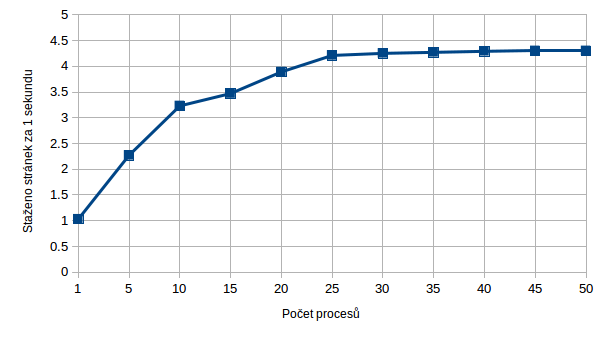
\includegraphics[width=1.0\textwidth]{obrazky-figures/graph_stahovani.png}
        \caption{Vliv počtu procesů na počet stažených stránek za jednu sekundu.}
    \end{center}
\end{figure}

\section{Nástroje pro kompresi dat}
Během výběru vhodného nástroje pro kompresi dat bylo nutné rozhodnout, který nástroj
je pro použití v~tomto projektu vhodnější. Doposud byly používány dva nástroje ke kompresi dat -- \textit{gzip}
a~\textit{xz}. Nástroj \textit{xz} využívá algoritmu \textit{lzma}. Pro zajímavost byl ke srovnání
přídán i populární nástroj \textit{zip}. Všechny nástroje byly spuštěny s~nejvyšší
úrovní komprese dat.

Vstupnímy daty pro tyto nástroje bylo 7 souborů o~velikosti 100 MB, 200 MB, 300 MB,
400 MB, 500 MB, 600 MB a~700 MB. Všechny tyto soubory obsahovaly stažené webové
stránky ve formátu WARC~(\ref{warc_format}). Měření probíhalo na stroji athena1.

Cílem měření výkonnosti těchto nástrojů a~efektivnosti algoritmů, které používají, bylo
zvolit nejvhodnější nástroj pro kompresi. Měřenými daty byla náročnost na procesor
během komprese a~dekomprese dat a~výsledná velikost archivu.

\subsection{Výsledky měření}
Na grafu~(\ref{graph:komprese}) lze vidět zatížení procesorů během komprese dat.
Nástroj \textit{gzip}  ve všech případech předčil nástroj \textit{zip}, přestože
oba nástroje měly velice podobné výsledky. Nástroj \textit{xz} klade výrazně
větší zátěž na procesor a~zpracování tak trvá mnohem déle.

\begin{figure}[H]
    \begin{center}
        \label{graph:komprese}
        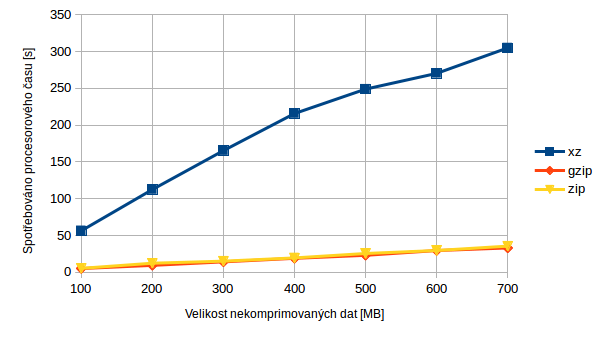
\includegraphics[width=1.0\textwidth]{obrazky-figures/graph_komprese.png}
        \caption{Procesorové zatížení během komprese dat.}
    \end{center}
\end{figure}

Graf~(\ref{graph:dekomprese}) vizualizuje výsledky měření náročnosti dekomprese na
procesor. Dekomprese je mnohem méně náročná a~největší úspěch zde má opět nástroj
\textit{gzip}, přestože \textit{zip} dosahuje podobných výsledků. Nástroj \textit{xz}
má opět nejhorší výsledek, ale faktem je, že čím větší je velikost dat, tím
se jeho celková náročnost blíží k~náročnosti ostatních nástrojů.

\begin{figure}[H]
    \begin{center}
        \label{graph:dekomprese}
        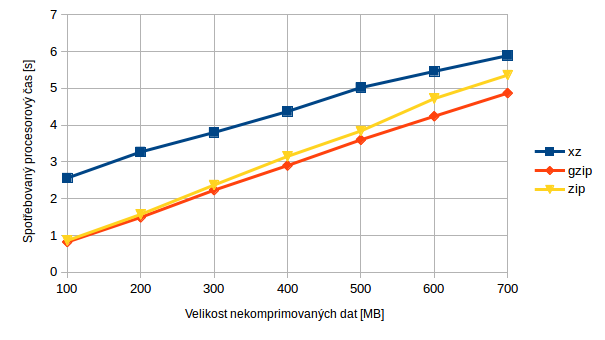
\includegraphics[width=1.0\textwidth]{obrazky-figures/graph_dekomprese.png}
        \caption{Procesorové zatížení během dekomprese dat.}
    \end{center}
\end{figure}

Důvodem, proč byl vybrán nástroj \textit{xz} ke kompresi dat, byla výsledná
velikost archivů. V~grafu~(\ref{graph:vysledna_velikost}) je vidět,
jak moc nástroj \textit{xz} v~tomto ohledu předčil nástroje \textit{gzip} a~\textit{zip}.
Nástroje \textit{gzip} a~\textit{zip} dosáhly v~tomto měření téměř totožných výsledků.

\begin{figure}[H]
    \begin{center}
        \label{graph:vysledna_velikost}
        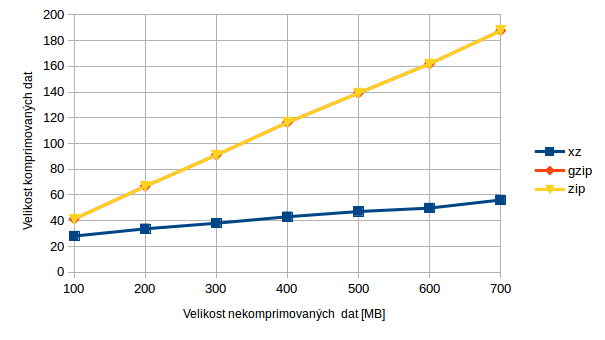
\includegraphics[width=1.0\textwidth]{obrazky-figures/graph_vysledna_velikost.png}
        \caption{Výsledná velikost komprimovaných dat.}
    \end{center}
\end{figure}

\section{Získání čistého textu, tokenizace a~vertikalizace}
Cílem k~efektivní práci těchto částí projektu je potřeba najít kompromis mezi
delší dobou zpracování a~vysokou paměťovou náročností. S~přibývajícím
počtem procesů roste nejen rychlost zpracování, ale i paměťová náročnost. Vše má své hranice a~záleží zejména na stroji, kde je nástroj spuštěn, při kolika procesech začne být
zpracování neefektivní z~důvodu nedostatku paměti nebo neschopnosti efektivně obsluhovat velké
množství procesů. Aby bylo možné rychlost zpracování porovnast s~původním
systémem, bylo nutné sáhnout po starších webových kolekcí, které byly přizpůsobeny pro
nástroj vertikalizátor.

Vešekeré měření včetně srovnání \textit{vertikalizátoru}~(\ref{vertikalizator}) a~současného systému probíhalo na
serveru athena1.

\subsection{Srovnání systémů}
Pro srovnání systémů byly vybrány balíčky o~přibližné velikosti 100 MB, 150 MB,
200 MB a~250 MB. Oba nástroje byly spuštěny bez detekce jazyka a~nový systém
byl spuštěn na 12 procesech (tento počet byl zvolen, protože byl v~době tvorby této
práce použit v~automatickém zpracování). Měřenými hodnotami byla reálná doba zpracování
a~procesorová náročnost.

Graf~(\ref{graph:graph_vertikalizator_vs_ja}) ukazuje výsledky srovnání obou nástrojů.
Z~hlediska procesorové náročnosti nový systém ukázal, že má ve většině případů horší výsledky
než původní vertikalizátor. Nový systém ale nepochybně předčil ten starý systém v~reálném
čase (dokud má stroj dostatek paměti a~více jader na procesoru nebo samotných procesorů). Pokud
je potřeba oba systémy porovnat při spuštění na jednom procesoru, lze z~grafů~(\ref{graph:graph_realny_cas_vertikalizace})
a~(\ref{graph:graph_procesorovy_cas_vertikalizace}) vyčíst, že nový systém lehce zaostává
za tím původním.

\begin{figure}[H]
    \begin{center}
        \label{graph:graph_vertikalizator_vs_ja}
        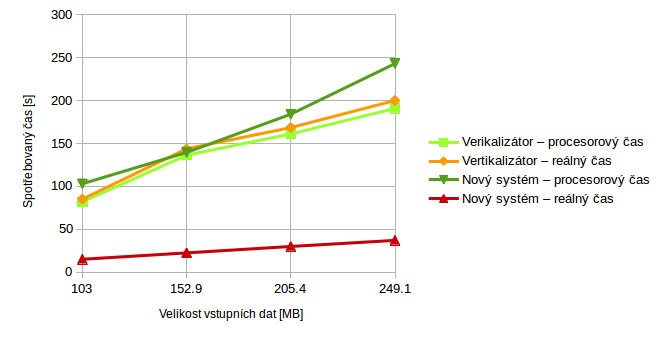
\includegraphics[width=1.0\textwidth]{obrazky-figures/graph_vertikalizator_vs_ja.png}
        \caption{Srovnání původního vertikalizátoru a~nového systému z~hlediska časové a~procesorové náročnosti.}
    \end{center}
\end{figure}

Na grafu~(\ref{graph:graph_realny_cas_vertikalizace}) je názorná ukázka toho, jak velký vliv má počet
procesů na celkovou rychlost zpracování. Z~grafu lze také vyčíst, že čím více je použito procesů,
tím méně naroste výkon s~dalším přidaným procesem. Z~toho důvodu je zbytečné spouštět
program s~příliš velkým počtem procesů, byť by na to stroj mohl mít výpočetní kapacitu.

\begin{figure}[H]
    \begin{center}
        \label{graph:graph_realny_cas_vertikalizace}
        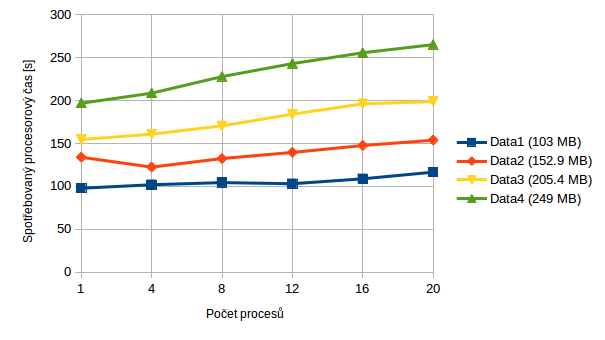
\includegraphics[width=1.0\textwidth]{obrazky-figures/graph_procesorovy_cas_vertikalizace.png}
        \caption{Vliv počtu procesů na celkovou procesorovou náročnost zpracování novým systémem.}
    \end{center}
\end{figure}

Vliv počtu procesů na celkovou spotřebu procesorového času není vůbec drastický. Vypočítaná data
jsou znázorněna grafem~(\ref{graph:graph_procesorovy_cas_vertikalizace}). Zajímavé je,
že čím větší je velikost zdrojových dat, tím větší vliv má i počet procesů na
celkovou náročnost výpočtu.

\begin{figure}[H]
    \begin{center}
        \label{graph:graph_procesorovy_cas_vertikalizace}
        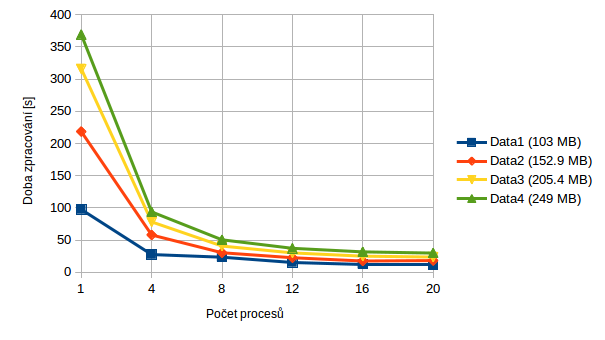
\includegraphics[width=1.0\textwidth]{obrazky-figures/graph_realny_cas_vertikalizace.png}
        \caption{Vliv počtu procesů na celkovou časovou náročnost zpracování novým systémem.}
    \end{center}
\end{figure}

Cenou za rychlejší zpracování je vyšší paměťová náročnost. Vztah počtu procesů na maximální
využití paměti během zpracování dat je znázorněn na grafu~(\ref{graph:graph_vertikalizace_pamet}).
Na grafu je znázorněno maximální využití paměti během procesu zpracování.

\begin{figure}[H]
    \begin{center}
        \label{graph:graph_vertikalizace_pamet}
        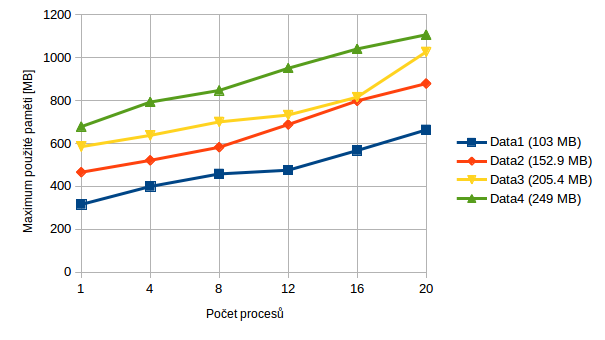
\includegraphics[width=1.0\textwidth]{obrazky-figures/graph_vertikalizace_pamet.png}
        \caption{Vliv počtu procesů na celkovou paměťovou náročnost zpracování novým systémem.}
    \end{center}
\end{figure}


\section{Tagging}
Měřenými hodnotami při provádění taggingu byly: procesorová náročnost, doba zpracování
a~množství využité paměti během zpracování. Vstupními daty byl soubor vertikalizovaných stránek
vytvořený během měření taggingu. Velikost vertikálního souboru byla 102 MB. Původní velikost
stažených dat (před provedením vertikalizace) byla 249 MB. Tento soubor obsahoval celkem
3408 stránek.

Bez zásahu do zdrojového kódu lze náročnost zpracování ovlivnit dvěma způsoby.
Prvním z~nich je počet stránek zpracovaných během jednoho spuštění taggingu. Druhý způsob
je počet procesů, které provádí tagging. Na následujících grafech je znázorněna závislost
nastavení těchto parametrů na celkovou zátěž kladenou na stroj athena1 během zpracování.
Jednotlivé funkce znázorněné v~grafu jsou počty stránek zpracovaných během jednoho spuštění
taggingu. Na ose X je poté znázorněn počet procesů použitých k~provedení taggingu a~na
ose Y je znázorněna výsledná zátěž.

Na grafu~(\ref{graph:graph_tagging_doba_zpracovani}) je znázorněna závislost počtu procesů
a~počtu zpracovaných stránek během jednoho spuštění taggingu na celkovou časovou náročnost
zpracování. Nejlepšího výsledku bylo dosaženo při použití 8 procesů a~zpracování 50
stránek během jednoho cyklu taggingu.

\begin{figure}[H]
    \begin{center}
        \label{graph:graph_tagging_doba_zpracovani}
        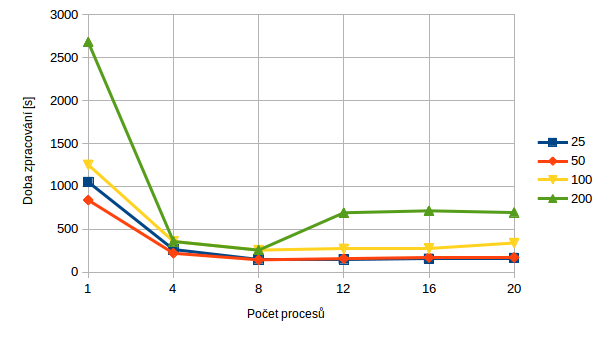
\includegraphics[width=1.0\textwidth]{obrazky-figures/graph_tagging_doba_zpracovani.png}
        \caption{Vliv počtu procesů na celkovou dobu zpracování novým systémem.}
    \end{center}
\end{figure}

Na grafu~(\ref{graph:graph_tagging_procesorovy_cas}) je zobrazena spotřeba procesorového času.
Nejlepších hodnot bylo vždy dosaženo při zpracování 50 stránek během jednoho spuštění taggingu.
Co se počtu procesorů týče, tak nejlepšího výsledku bylo dosaženo při použití 4 procesů.

\begin{figure}[H]
    \begin{center}
        \label{graph:graph_tagging_procesorovy_cas}
        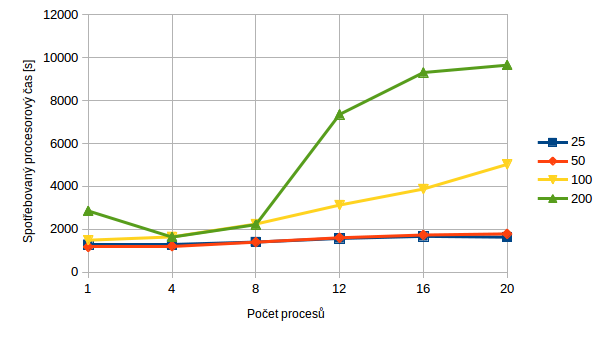
\includegraphics[width=1.0\textwidth]{obrazky-figures/graph_tagging_procesorovy_cas.png}
        \caption{Vliv počtu procesů na celkovou procesorovou náročnost zpracování novým systémem.}
    \end{center}
\end{figure}

Stejně jako u~vertikalizace, i zde spolu s~počtem procesů roste velikost potřebné paměti.
Graf~(\ref{graph:graph_tagging_pamet}) zobrazuje vliv počtu procesů a~počtu zpracovaných stránek
během jednoho spuštění taggeru. Nejlepších výsledků bylo dosaženo při zpracování jedním procesem
s~25 stránkami zpracovanými během jednoho cyklu taggingu.

\begin{figure}[H]
    \begin{center}
        \label{graph:graph_tagging_pamet}
        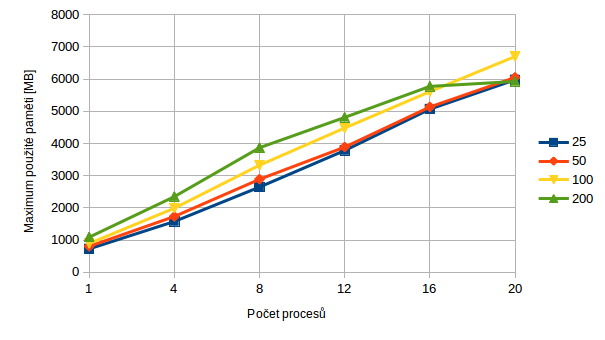
\includegraphics[width=1.0\textwidth]{obrazky-figures/graph_tagging_pamet.png}
        \caption{Vliv počtu procesů na celkovou paměťovou náročnost zpracování novým systémem.}
    \end{center}
\end{figure}

\chapter{Závěr}
Byla vytvořena řada nových nástrojů umožňujících automatickou kolekci, stahování a~zpracování dat. Nástroje byly vyvíjeny a~testovány zejména nad slovenskými a~českými zpravodajskými deníky, ale je možné je použít na zpracování
všech HTML stránek.

Některé nástroje v~tomto projektu již byly vyvinuty, v~takových případech tento projekt
nabízí alternativu k~těmto nástrojům. Nové nástoje, které jsou v~této práci popsané,
umožňují maximální využití zdrojů stroje, na kterém jsou spuštěny, a~proto jsou
schopny na strojích, které mají více jader na procesoru nebo dokonce více procesorů,
zpracovat data mnohem rychleji. Ne příliš vysokou cenou za tuto rychlost je vyšší
zátěž na procesor a~množství potřebné paměti. Díky nástroji \textit{xz} je
zde i větší úspora úložného prostoru dat než u~dřívějšího způsobu archivace pomocí
nástroje \textit{gzip}.

Další nezanedbatelnou výhodou je umožnění rychlé výměny nástrojů bez nutnosti přepisovat veškěré
zdrojové kódy v~případě, že se některý z~použitých nástrojů ukáže jako méně vhodným.
Na rozdíl od předchozích projektů, tento umožňuje zpracovat data v~českém, anglickém a~slovenském jazyce. Není vyloučeno ani zpracování dalších jazyků v~případě, že se
k~nim dodá jazykový model. Na rozdíl od \textit{vertikalizátoru}~(\ref{vertikalizator}),
který je doposud používán kromě jiného k~detekci jazyka stránky, je nový systém schopen zpracovat
nejen archiv, obsahující stránky v~různých jazycích, ale dokonce i samotnou stránku psanou
ve více než jednom jazyce. Tato schopnost zpracovat vícejazyčné texty dává novému
systému obrovskou výhodu při použití ke zpracování vícejazyčných webových stránek,
komentářů, diskuzí nebo zpracování různých recenzí a~obsahu sociálních médií, kde se běžně
oběvuje více jazyků.

Nevýhodou tohoto systému je skutečnost, že zpracování výstupních dat této práce dalšími nástroji
je možné až po úpravě těchto nástrojů tak, aby byly schopny zpracovat nový formát dat.
Naštěstí se nejedná o~žádné zásadní úpravy a~lze tento problém řešit i jiným způsobem. Jedním ze
způsobů je implementace podpory formátu dat, který využívají dané nástroje. Tento projekt
lze tedy spustit tak, aby výstupní data odpovídala formátu, který se doposud používal.
Za tuto podporu se platí ztrátou některých výhod, jako je například detekce
jazyka. Druhou možností je vytvoření jednoduchých programů, které převedou nový formát
do starého a~po použití potřebných nástrojů zase zpět. Tímto se ale ztrácí úspora času
a~jednoduchost použití tohoto systému.
%=========================================================================


  % Kompilace po částech (viz výše, nutno odkomentovat)
  % Compilation piecewise (see above, it is necessary to uncomment it)
  %\subfile{projekt-01-uvod-introduction}
  % ...
  %\subfile{chapters/projekt-05-conclusion}


  % Pouzita literatura / Bibliography
  % ----------------------------------------------
\ifslovak
  \makeatletter
  \def\@openbib@code{\addcontentsline{toc}{chapter}{Literatúra}}
  \makeatother
  \bibliographystyle{bib-styles/slovakiso}
\else
  \ifczech
    \makeatletter
    \def\@openbib@code{\addcontentsline{toc}{chapter}{Literatura}}
    \makeatother
    \bibliographystyle{bib-styles/czechiso}
  \else
    \makeatletter
    \def\@openbib@code{\addcontentsline{toc}{chapter}{Bibliography}}
    \makeatother
    \bibliographystyle{bib-styles/englishiso}
  %  \bibliographystyle{alpha}
  \fi
\fi
  \begin{flushleft}
  \bibliography{projekt-20-literatura-bibliography}
  \end{flushleft}

  % vynechani stranky v oboustrannem rezimu
  % Skip the page in the two-sided mode
  \iftwoside
    \cleardoublepage
  \fi

  % Prilohy / Appendices
  % ---------------------------------------------
  \appendix
\ifczech
  \renewcommand{\appendixpagename}{Přílohy}
  \renewcommand{\appendixtocname}{Přílohy}
  \renewcommand{\appendixname}{Příloha}
\fi
\ifslovak
  \renewcommand{\appendixpagename}{Prílohy}
  \renewcommand{\appendixtocname}{Prílohy}
  \renewcommand{\appendixname}{Príloha}
\fi
%  \appendixpage

% vynechani stranky v oboustrannem rezimu
% Skip the page in the two-sided mode
%\iftwoside
%  \cleardoublepage
%\fi

\ifslovak
%  \section*{Zoznam príloh}
%  \addcontentsline{toc}{section}{Zoznam príloh}
\else
  \ifczech
%    \section*{Seznam příloh}
%    \addcontentsline{toc}{section}{Seznam příloh}
  \else
%    \section*{List of Appendices}
%    \addcontentsline{toc}{section}{List of Appendices}
  \fi
\fi
  \startcontents[chapters]
  \setlength{\parskip}{0pt}
  % seznam příloh / list of appendices
  % \printcontents[chapters]{l}{0}{\setcounter{tocdepth}{2}}

  \ifODSAZ
    \setlength{\parskip}{0.5\bigskipamount}
  \else
    \setlength{\parskip}{0pt}
  \fi

  % vynechani stranky v oboustrannem rezimu
  \iftwoside
    \cleardoublepage
  \fi

  % Přílohy / Appendices
  % Tento soubor nahraďte vlastním souborem s přílohami (nadpisy níže jsou pouze pro příklad)
% This file should be replaced with your file with an appendices (headings below are examples only)

% Umístění obsahu paměťového média do příloh je vhodné konzultovat s vedoucím
% Placing of table of contents of the memory media here should be consulted with a supervisor
%\chapter{Obsah přiloženého paměťového média}

%\chapter{Manuál}

%\chapter{Konfigurační soubor} % Configuration file

%\chapter{RelaxNG Schéma konfiguračního souboru} % Scheme of RelaxNG configuration file
\chapter{Plakát}
Obrázek \ref{plakat} je zmenšený plakát, který byl vytvořen v rámci této práce. V elektronické
verzi je plakát ve formátu SVG (Scalable Vector Graphics).
\begin{figure}[p]
    \label{plakat}
    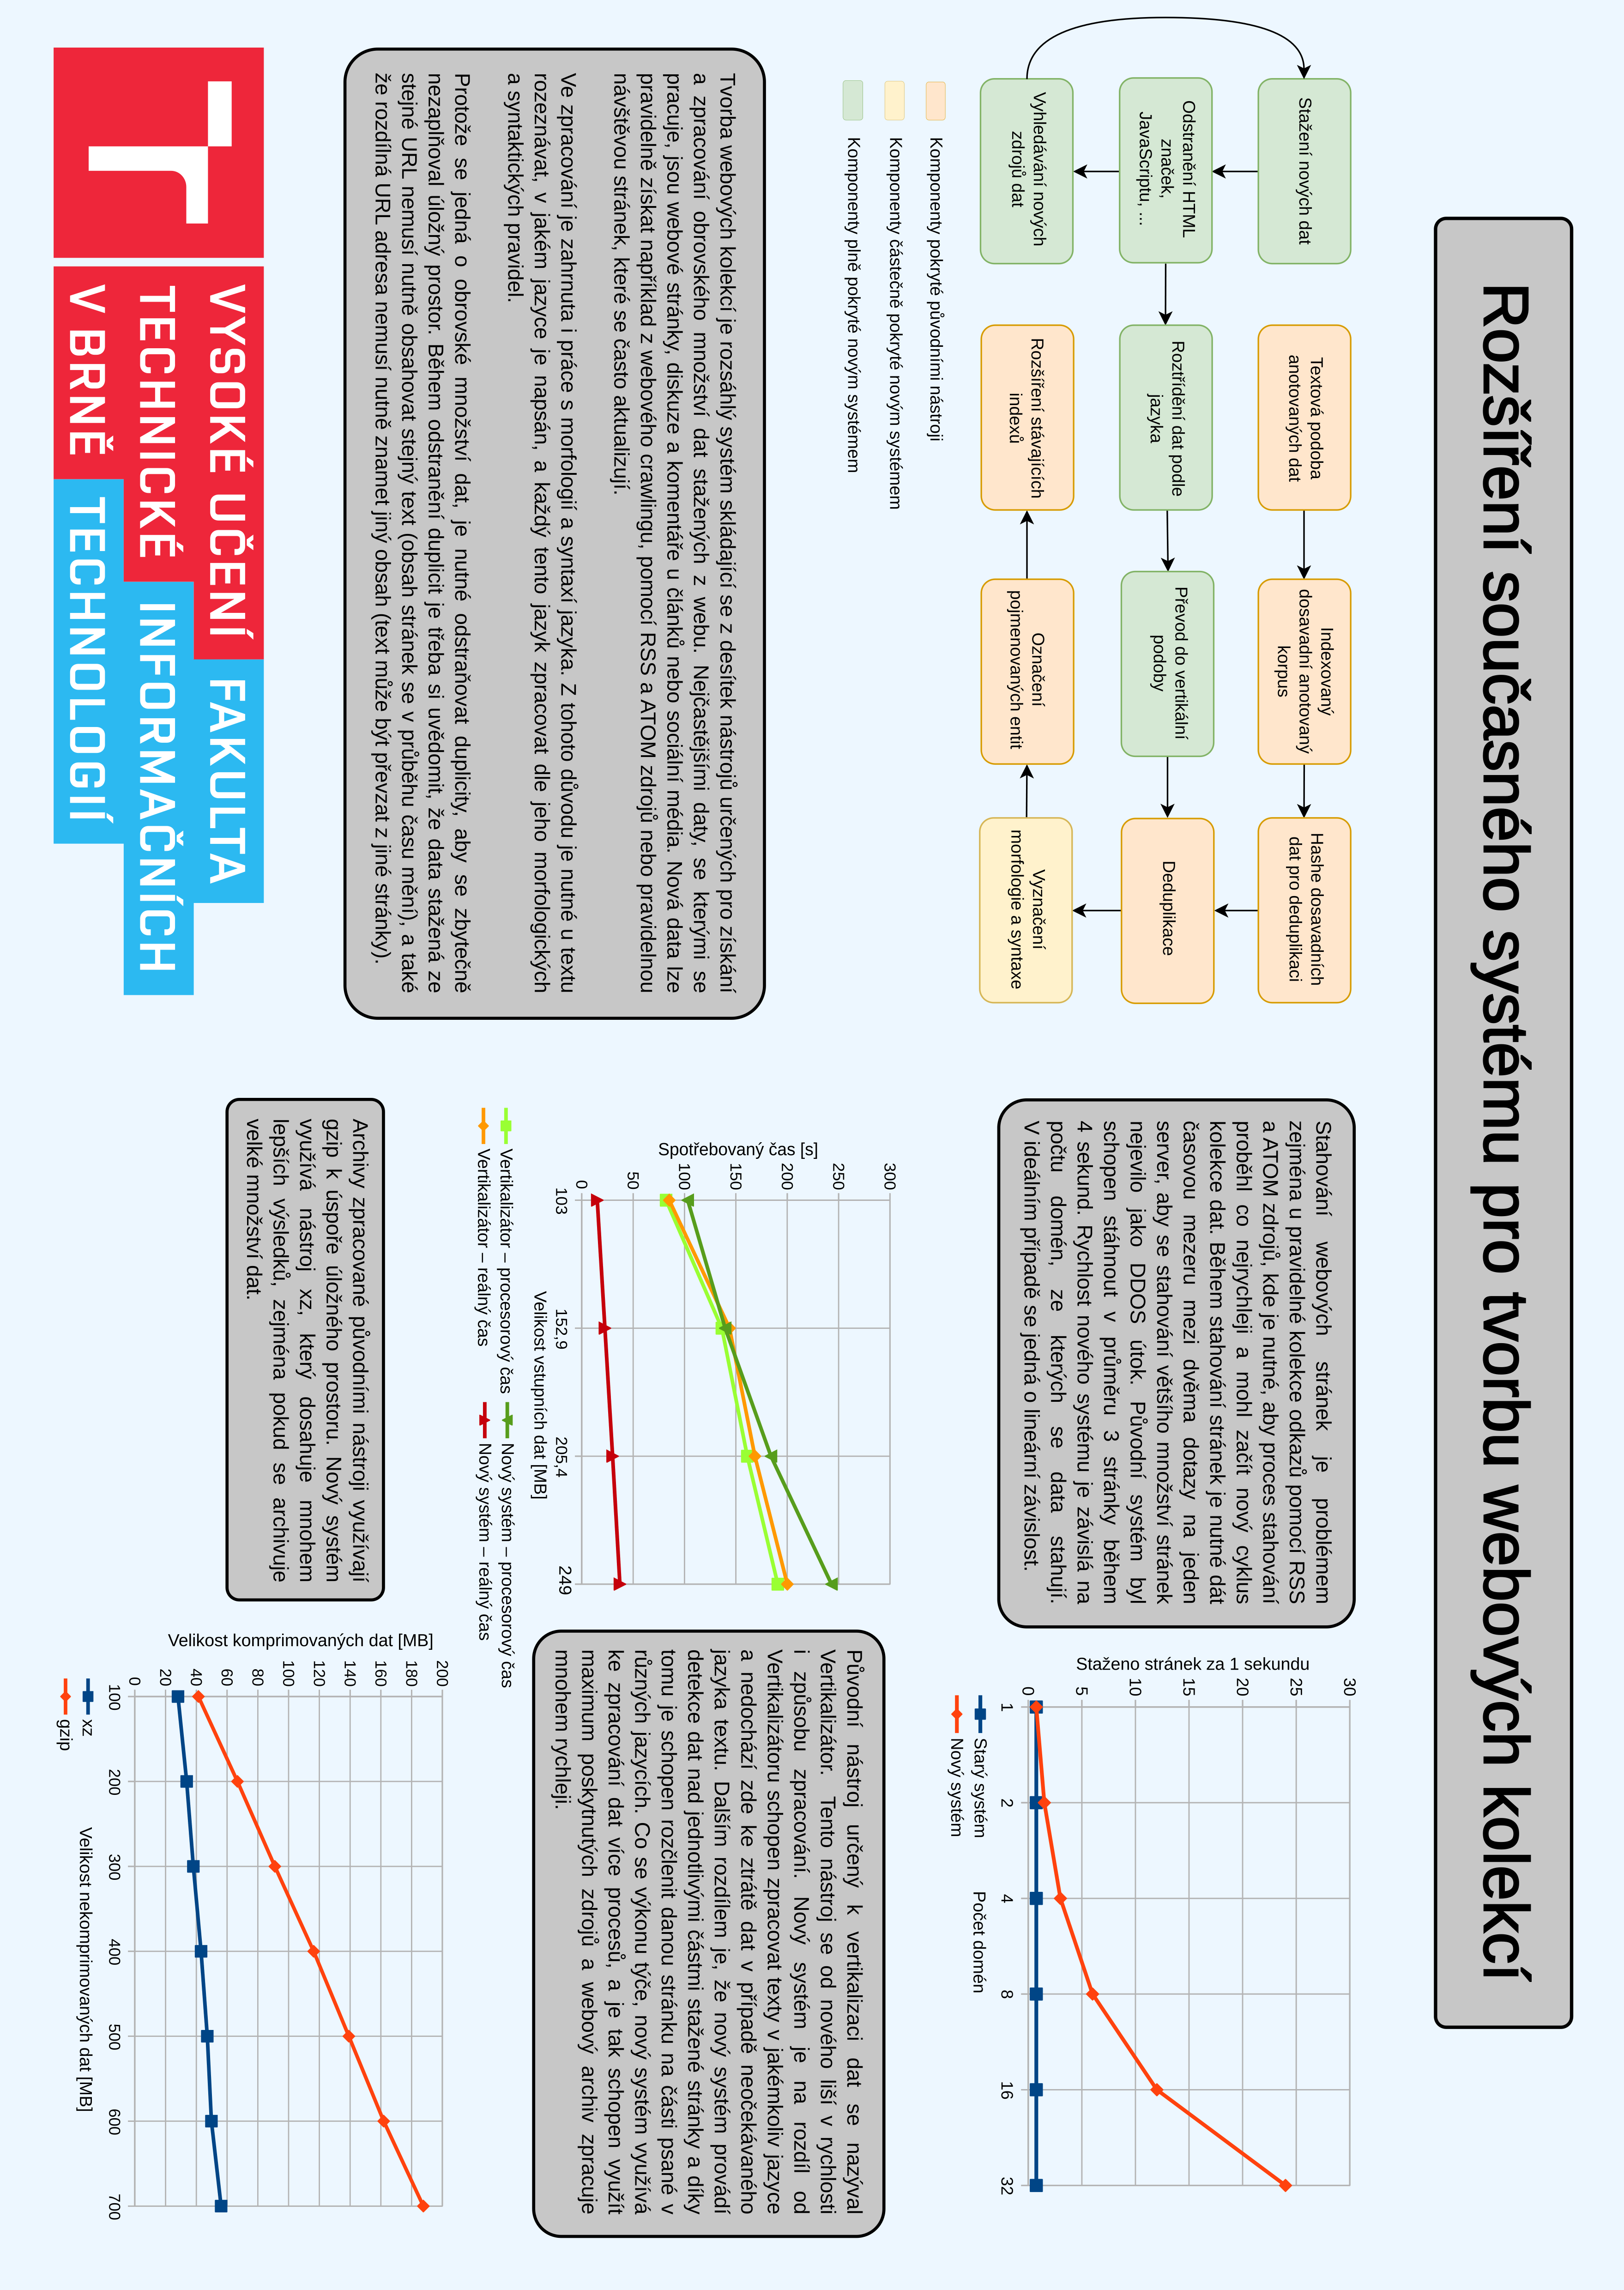
\includegraphics[height=\paperwidth,width=\paperwidth,keepaspectratio]{obrazky-figures/plakat.png}
    \caption{Plakát stručně popisující projekt.}
\end{figure}

  % Kompilace po částech (viz výše, nutno odkomentovat)
  % Compilation piecewise (see above, it is necessary to uncomment it)
  %\subfile{projekt-30-prilohy-appendices}

\end{document}
